\documentclass[11pt]{article}
\ifdefined\pdftrailerid\pdftrailerid{}\fi
\newcommand{\DoNotLoadEpstopdf}{}
\usepackage[T1]{fontenc}
\usepackage{lmodern,microtype,amsmath,amssymb,amsthm,mathtools,booktabs,array,tikz}
\usetikzlibrary{arrows.meta}
\usepackage[a4paper,hmargin=25mm,vmargin=23mm]{geometry}
\usepackage[hidelinks,bookmarksnumbered]{hyperref}
\numberwithin{equation}{section}
\newtheorem{theorem}{Theorem}[section]
\newtheorem{proposition}[theorem]{Proposition}
\newtheorem{lemma}[theorem]{Lemma}
\newtheorem{corollary}[theorem]{Corollary}
\newtheorem{localcorollary}{Corollary}[theorem]
\renewcommand{\thelocalcorollary}{\thetheorem\alph{localcorollary}}
\theoremstyle{definition}
\newtheorem{definition}[theorem]{Definition}
\theoremstyle{remark}
\newtheorem{remark}[theorem]{Remark}
\newtheorem{example}[theorem]{Example}

\newcommand{\R}{\mathbb{R}}
\newcommand{\Q}{\mathbb{Q}}
\newcommand{\Z}{\mathbb{Z}}
\newcommand{\dd}{\mathrm{d}}
\newcommand{\eps}{\varepsilon}
\newcommand{\sgn}{\operatorname{sgn}}
\newcommand{\HH}{H_{\mathrm{hyp}}}
\newcommand{\D}{\mathcal{D}}
\newcommand{\M}{\mathcal{M}}
\newcommand{\J}{\mathcal{J}}
\newcommand{\ind}{\mathbf{1}}

\setlength{\emergencystretch}{1em}
\raggedbottom

\setcounter{tocdepth}{1}

\hypersetup{pdfauthor={Haibo Lu},pdftitle={Relative return gaps and a 7/2 asymptotic lower bound for hyperbolic limit cycles in classical Lienard systems},
pdfsubject={Finite entrance lists and exact primitive degree}}
\title{Relative return gaps and a $7/2$ asymptotic lower bound\\ for hyperbolic limit cycles in classical Li\'enard systems}
\author{Haibo Lu\\[2pt]
\small Shanghai Institute of Technology, Shanghai 201418, China\\
\small Correspondence: \nolinkurl{luhaibo1985@gmail.com}\\
\small ORCID: \href{https://orcid.org/0009-0000-2717-5968}{0009-0000-2717-5968}}
\date{24 November 2026}
\begin{document}
\maketitle
\begin{abstract}
For the classical Li\'enard equation $\ddot x+F'(x)\dot x+x=0$, let $n$
be the exact degree of the polynomial $F$. For every $n\ge14$ we
construct a nonempty open set of coefficients for which at least
$\lceil(7n-48)/2\rceil$ geometrically distinct hyperbolic limit cycles
coexist. The asymptotic coefficient of this bound is $7/2$, compared
with one in the $n-2$ construction of De Maesschalck and Huzak.

After reflecting the left half-plane and reversing time there, we compare
lower-axis hits for three families of trajectories. One starts on the
positive $y$-axis. The other two enter from spatial infinity with
positive or negative limiting ordinate. A shallow well, a local maximum
followed outwards by a nearby minimum on one reflected profile, adds
three, three and one sign changes to the respective lists. To turn
the incoming comparisons into return brackets we add higher powers that create a distant
maximum on each side. Tracing a finite entrance backwards past this
maximum takes it to the upper axis. Ratios of exponentially small gaps
from a matched reference determine an $o(1)$ adjustment of the opposite
entrance ordinate that gives exactly the same upper crossing. This
preserves every strict comparison in a fixed finite list. A single
change of the linear coefficient gives hyperbolic cycles in the
resulting brackets. The construction retains the cycles in a fixed
compact region and gains seven cycles for every two additional degrees.
\end{abstract}

\section{Coexisting cycles at fixed primitive degree}\label{sec:intro}
How many limit cycles can coexist when the restoring force is linear and the polynomial primitive $F$ has exact degree $n$? We write the scalar
equation $\ddot x+F'(x)\dot x+x=0$ as
\begin{equation}\label{eq:lienard}
 \dot x=y-F(x),\qquad \dot y=-x,\qquad
 F(x)=\sum_{j=1}^n a_jx^j,\qquad a_n\ne0 .
\end{equation}
A vertical translation removes the constant term. The remaining
coefficients are unrestricted. Throughout, $n$ is the exact degree
of the primitive $F$, so the damping has degree $n-1$.
Let $H(n)$ be the supremum, over all fields~\eqref{eq:lienard} of exact
degree $n$, of the number of geometrically distinct isolated periodic
orbits in one field. Define $\HH(n)$ by counting hyperbolic orbits
(transverse multiplier different from one) and $H_{\le}(n)$ by counting
isolated orbits over degrees at most $n$. Thus
$\HH(n)\le H(n)\le H_{\le}(n)$. The following bound comes from
placing successive families of cycles on separated spatial scales.

\begin{theorem}[Exact-degree lower bound]\label{thm:main-asymptotic}
For every integer $n\ge14$ there is a nonempty open subset of
$\{(a_1,\ldots,a_n)\in\R^n:a_n\ne0\}$ on which every field~\eqref{eq:lienard}
has at least $L(n)$ geometrically distinct hyperbolic limit cycles, where
\begin{equation}\label{eq:parity-bounds}
 L(n)=\left\lceil\frac{7n-48}{2}\right\rceil
 =\begin{cases}(7n-48)/2,& n\ \mathrm{even},\\ (7n-47)/2,& n\ \mathrm{odd}.\end{cases}
\end{equation}
In particular $\liminf_{n\to\infty}\HH(n)/n\ge7/2$. By density, the
open set at each degree contains a rational coefficient vector.
\end{theorem}

\begin{corollary}[Low degrees of the octic construction]\label{cor:octic-low}
At exact degrees $8,10,11,12,13$ there are nonempty open sets with at
least $9,10,15,18,22$ coexisting hyperbolic cycles, respectively.
\end{corollary}
Section~\ref{subsec:prove-asymptotic} proves the corollary with zero or
one well insertion. The first insertion raises the odd count from
fifteen at eleven to twenty-two at thirteen and the even count from
eighteen at twelve to twenty-five at fourteen.

\paragraph{The classical degree problem.}
Lins, de Melo and Pugh proposed a maximum of $k$ cycles at degrees
$2k+1$ and $2k+2$~\cite[pp.~335--336]{LMP1977}. A quartic has at most
one cycle, hyperbolic when present~\cite[Theorem~1.1]{LiLlibre2012}.
Odani's odd quintics attain two hyperbolic cycles~\cite{Odani1996}.
The upper bounds of Rychkov, Li and Lu, and Chen, Chen and Xiao concern
odd quintics, a given nondegenerate slow--fast cycle, and the small-parameter
regime for a fixed quintic, respectively~\cite{Rychkov1975,LiLu2014,CCX2026}.
With the upper bound stated in the quintic preprint
\cite[Theorem~1.1]{OpenAIQuintic2026}, Odani's lower example would give
$H_{\le}(5)=H(5)=\HH(5)=2$.

Dumortier, Panazzolo and Roussarie obtained four cycles at primitive
degree seven, disproving the proposed maximum~\cite[Theorems~1.1 and
1.3]{DPR2007}. De Maesschalck and Dumortier used a canard orbit through
a prescribed section height to obtain $\lfloor(n-1)/2\rfloor+2$
hyperbolic cycles at every exact $n\ge6$~\cite[Theorem~2 and
Proposition~1]{DMD2011}. De Maesschalck and Huzak raised the
hyperbolic bound to $n-2$ for both parities~\cite[Theorem~1]{DMH2015}.
Their near-center construction uses a monotone positive branch of the even primitive and one slow divergence integral.
Its nonzero first-order term has at most $n-3$ positive zeros, and their
construction includes a reference cycle. They conjectured $n-2$ as a
maximum for the classical system~\cite[Proposition~3 and Remark~2]{DMH2015}.

At each exact $n\ge6$ the Palomar repository preprint constructs
$\lfloor(n-1)/2\rfloor+4$ isolated cycles, including six throughout
a sextic coefficient box and seven for a specified septic
\cite[Theorems~1--2, Corollary~19 and Proposition~21]{Palomar2026}.
These are already counterexamples to the proposed $n-2$ maximum at
degrees six through nine. The preprint's strict sign brackets give
the same counts of hyperbolic cycles in nearby fields by
Proposition~\ref{prop:sard}(i). The first improvement over these
combined bounds is from seven to nine at degree eight
(Table~\ref{tab:exact-degrees}). The octic construction in
Section~\ref{sec:wells} compares \emph{actions}, the magnitudes of the
reduced slow divergence integrals over the slow arcs shared by a trajectory
and its reference.
The supplement uses validated sextic shooting and entrance data to
obtain ten cycles at degree nine and to improve the octic counts
from ten to fourteen at degree ten and from eighteen to nineteen at
degree twelve~\cite[\S\S S3--S5]{ElectronicSupplement}. In the supplement's
notation, $\eta>0$ controls the splitting of a stationary inflection into
two folds. For every sufficiently small value, three matching equations
and one regular choice of the linear coefficient give nineteen coexisting
hyperbolic cycles in one field. Persistence gives a nonempty open set,
which contains rational members by density. The supplement also specifies
two rational degree-twelve fields. One has exactly five hyperbolic cycles
in its weak full-return domain. The other has at least six, including a
repelling outer cycle
\cite[Remark~SA.1 and Proposition~SB.1]{ElectronicSupplement}.

\begin{table}[htbp]
\centering\small
\caption{Lower bounds at exact primitive degree. The published bounds are
Odani's at five and De Maesschalck--Huzak's thereafter. The comparison
row also uses Proposition~\ref{prop:sard}(i) on the Palomar brackets.
S1.1 and S1.2 are the supplement's theorem and proposition.
A denotes an analytic proof with finite algebraic estimates.
V also uses validated sextic trajectory enclosures. In the proof row,
\emph{core} and \emph{odd} refer to Section~\ref{subsec:prove-asymptotic},
with $t$ inserted wells.}\label{tab:exact-degrees}
\smallskip\setlength{\tabcolsep}{3.5pt}
\begin{tabular}{@{}l*{9}{c}@{}}
\toprule
$n=\deg F$ &5&6&7&8&9&10&11&12&13\\
\midrule
Published, hyperbolic&2&4&5&6&7&8&9&10&11\\
Palomar preprint, isolated&--&6&7&7&8&8&9&9&10\\
Hyperbolic comparison&2&6&7&7&8&8&9&10&11\\
This work, hyperbolic&2&6&7&9&10&14&15&19&22\\
Gain over the comparison&0&0&0&2&2&6&6&9&11\\
\addlinespace
Statement&\hyperref[thm:weak]{A.1(iii)}&S1.2&S1.2&\ref{cor:octic-low}&S1.2&S1.2&\ref{cor:octic-low}&S1.1&\ref{cor:octic-low}\\
Evidence&A&V&V&A&V&V&A&V&A\\
Proof&$d=2$&S3.1&S3.1&\hyperlink{octic-core}{core}&S5.2&S4&\hyperlink{odd-closure}{odd, $t=0$}&S5.1&\hyperlink{odd-closure}{odd, $t=1$}\\
\bottomrule
\end{tabular}
\end{table}


For unrestricted planar polynomial fields of total degree at most $D$,
the multiple-center construction of Christopher and Lloyd~\cite[\S3]{CL1995},
with the count corrected by Li, Chan and Chung~\cite[Proposition~5]{LCC2002},
gives a lower bound of order $D^2\log D$. Han and Li sharpened the
asymptotic bound for all large degrees~\cite{HL2012}. Within a single nest
around one equilibrium, De Maesschalck and Torregrosa obtain at least
$(D-1)^2/2$ isolated cycles at odd degree $D$ with two variable polynomial
components~\cite[Theorems~1 and~4, system~(1)]{DMT2025}. The classical field~\eqref{eq:lienard}
has total degree $D=n$ and fixed second component $-x$. Every cycle
surrounds its sole equilibrium, the origin. Smale discusses
this subclass after his general degree question~\cite[Problem~13,
second version, (4)--(5)]{Smale1998}. Cen, Chen, Tian
and Zhao proposed a maximum of $k-1$ cycles when $F$ has exactly $k$
nonzero monomials~\cite{Cen2026}. For trinomials with two
odd powers below the leading even power $x^{2N}$ and opposite signs
on the odd coefficients, Chen, Jin, Li and Zhou obtain at least two
cycles for suitable coefficients and exponents at every $N\ge3$.
At $N=5$ they construct three hyperbolic cycles at degree ten, exceeding
the proposed maximum for $k=3$~\cite[Theorems~1.1--1.2 and \S3]{CJLZ2026}.
Table~\ref{tab:exact-degrees} fixes the degree and allows all lower powers.

\paragraph{From entrance comparisons to closed orbits.}
Reflect the left half-plane and reverse time there so that both
half-orbits run forward in $x>0$. For a launch at $(0,h)$ with $h>0$,
write $-w_+(h)$ and $-w_-(h)$ for the first hits on the negative
$y$-axis. Equality closes an orbit. Our first list compares the two
hit magnitudes at a sequence of upper-axis launches. For the other
two lists, prescribe the limiting ordinate $y$ of a trajectory as
$x\to+\infty$ on each reflected side and follow it inwards to the
lower axis. We call the trajectory a positive or negative entrance
according to the sign of $y$. In a fold window an upper launch and a
positive entrance reach different rising branches and accumulate
different slow divergence integrals. A negative entrance crosses the
whole profile, and its lower hit records the drift during that flight
(Figure~\ref{fig:mechanisms}(a)).

Closing the two sides in one polynomial requires both the upper-axis
crossing and the gaps from a common reference there. Local canard
transition maps describe how a gap depends on the entrance point.
Dumortier and Roussarie give smooth exponential
actions for the section maps in a two-parameter unfolding and derive
entrance-derivative asymptotics~\cite[\S2, Definition~2.1, (5)--(7),
Remark~5.2]{DR2007}. At a matched pair they rescale the two entrance coordinates by $\epsilon$ and expand their actions, obtaining exponential terms controlled by the entrance derivatives~\cite[\S6, (22)--(24)]{DR2007}. De Maesschalck, Dumortier and Roussarie write the
signed separation from a reference center manifold as an exponential
whose action depends smoothly on the entrance
\cite[\S2.3, (1)]{DMDR2023}. Their 2025 sequel treats local cyclicity
for planar two-layer canard cycles with specified layers and connections
\cite[p.~1]{DMDR2025}. For a smooth exponential action, differentiation
in the entrance coordinate already gives a local log-gap ratio.

The entry--exit integral relates accumulated attraction to subsequent
repulsion~\cite[(1.4)]{DMS2016}. Huzak, Jard\'on-Kojakhmetov and Kuehn
show that along a control curve the exit ordinate tracks a function
of the entrance, the slow relation function. The approximation has absolute $o(1)$ error on the prescribed compact
intervals. In the regime with a threshold, entrances below it follow
the slow relation and those above it have a common limiting exit
\cite[author version~2, Proposition~2]{HJK2025}.

We add higher powers to the input polynomial to form a distant
maximum on each reflected side (Figure~\ref{fig:mechanisms}(b)). A
launch on a finite exterior section approximates the original entrance
from infinity when followed inwards. Traced backwards, the same arc
reaches the outer falling branch, passes its maximum and hits the
positive $y$-axis. Thus the incoming comparison becomes a comparison
of half-returns once the two upper hits agree. Write $R$ for the
exterior length, $m$ for the even input degree and $z=|x|/R$. On each side
we trace a reference arc backwards from the lower axis. Two
coefficients make the reference arcs meet at the same upper-axis point
and match one pair of entrances on the section $z=1/2$. Their
\emph{physical ordinates} are $y_+=\Delta$ on the positive side
and $y_-=0$ on the negative side. Other ordinates a bounded physical
distance apart differ by only $O(\tau^m)$ in the scaled height
$t=y/R^m$, where $\tau=1/R$.
The error bound for the first action expansion at the maximum exceeds this scale.
Proposition~\ref{prop:cap-transfer}, formula~\eqref{eq:cap-fine},
shows that the scaled log ratio of gaps from this reference has a
strictly positive limiting slope in the physical entrance ordinate.
It pairs $y$ with $y-\Delta+o(1)$ on the other side at an \emph{exactly}
common upper crossing. Every strict sign in a fixed finite list thus
survives in one polynomial, and compact convergence preserves earlier
hyperbolic cycles in a fixed disk. For highest odd degree $j=m-1$
or $m-3$ the output has exact degree
$\max(m+2,j+4)$. The outer length depends on the list and its sign
margins. Example~\ref{ex:repelling} illustrates how later expansion
can erase the entrance separation.

\begin{figure}[ht]
\centering
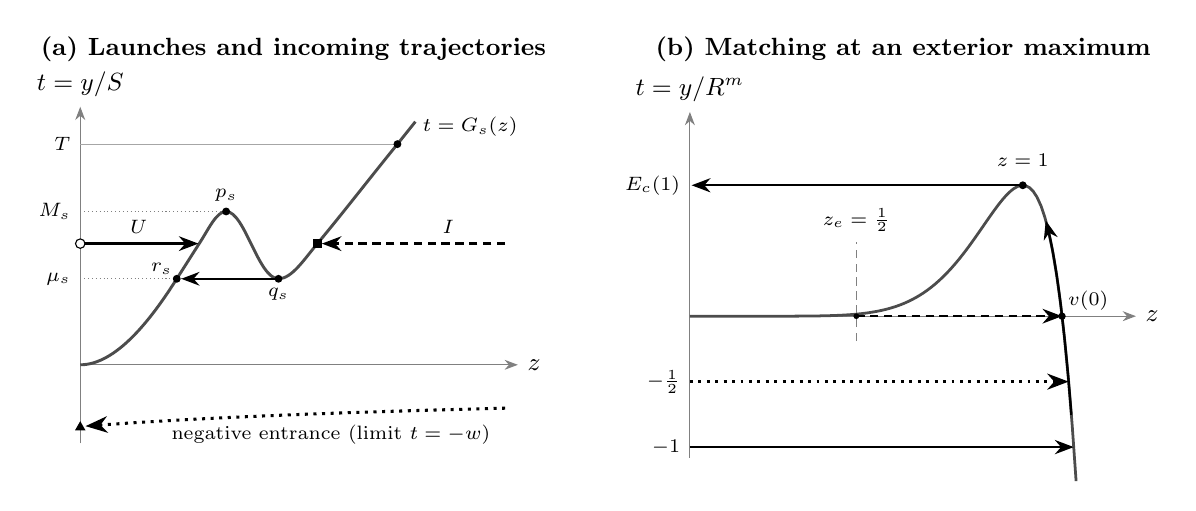
\begin{tikzpicture}[>=Stealth, font=\small, scale=0.95]
  % Left panel: three inner regimes
  \begin{scope}[shift={(0,0)}]
    \node[anchor=south, font=\bfseries\small] at (2.85,3.92) {(a) Launches and incoming trajectories};
    \draw[->,gray] (0,-1.05) -- (0,3.45) node[above,black] {$t=y/S$};
    \draw[->,gray] (0,0) -- (5.85,0) node[right,black] {$z$};
    % Profile G_s(z) with one fold window [mu_s, M_s]
    \draw[line width=1.05pt, black!70]
      (0,0) .. controls (0.48,0) and (0.95,0.61) .. (1.29,1.15)
      .. controls (1.38,1.29) and (1.50,1.48) .. (1.59,1.62)
      .. controls (1.72,1.82) and (1.82,2.05) .. (1.95,2.05)
      .. controls (2.20,2.05) and (2.38,1.15) .. (2.65,1.15)
      .. controls (2.83,1.15) and (3.00,1.42) .. (3.17,1.62)
      .. controls (3.52,2.04) and (3.85,2.47) .. (4.24,2.95)
      -- (4.48,3.25);
    \node[right, font=\scriptsize] at (4.45,3.18) {$t=G_s(z)$};
    % Reference T
    \draw[thin, gray!70] (0,2.95) -- (4.24,2.95);
    \node[left, font=\scriptsize] at (0,2.95) {$T$};
    \fill (4.24,2.95) circle (1.5pt);
    % Window levels M_s and mu_s
    \draw[densely dotted, gray] (0,2.05) -- (1.95,2.05);
    \draw[densely dotted, gray] (0,1.15) -- (2.65,1.15);
    \node[left, font=\scriptsize] at (0,2.05) {$M_s$};
    \node[left, font=\scriptsize] at (0,1.15) {$\mu_s$};
    % Jump from minimum q_s to landing r_s
    \draw[->, thick, black] (2.63,1.15) -- (1.35,1.15);
    \fill (2.65,1.15) circle (1.5pt) node[below, font=\scriptsize] {$q_s$};
    \fill (1.95,2.05) circle (1.5pt) node[above, font=\scriptsize] {$p_s$};
    \fill (1.29,1.15) circle (1.5pt) node[above left, inner sep=1.5pt, font=\scriptsize] {$r_s$};
    % 1. Trapped upper launch (solid + circle)
    \draw[->, line width=0.9pt] (0.05,1.62) -- (1.58,1.62);
    \fill[white] (0,1.62) circle (1.8pt); \draw (0,1.62) circle (1.8pt);
    \node[above, font=\scriptsize] at (0.78,1.63) {$U$};
    % 2. Positive incoming ray (dashed + square)
    \draw[->, densely dashed, line width=0.9pt] (5.68,1.62) -- (3.23,1.62);
    \fill ([xshift=-1.8pt,yshift=-1.8pt]3.17,1.62) rectangle ++(3.6pt,3.6pt);
    \node[above, font=\scriptsize] at (4.92,1.63) {$I$};
    % 3. Negative incoming flight (dotted + triangle)
    \draw[->, dotted, line width=1.1pt] (5.68,-0.58) .. controls (3.6,-0.63) and (1.7,-0.70) .. (0.07,-0.82);
    \node[below, font=\scriptsize] at (3.35,-0.68) {negative entrance (limit $t=-w$)};
    \fill (0,-0.82) ++(-2pt,-1.6pt) -- ++(4pt,0) -- ++(-2pt,3.5pt) -- cycle;
  \end{scope}

  % Limiting profile for m=8 and c=5. Axes are affine in z and t.
  \begin{scope}[shift={(8.15,0)}]
    \node[anchor=south, font=\bfseries\small] at (2.85,3.92) {(b) Matching at an exterior maximum};
    \begin{scope}[shift={(0,0.65)},x=4.45cm,y=1.75cm]
      \draw[->,gray] (0,-1.08) -- (0,1.56) node[above,black] {$t=y/R^m$};
      \draw[->,gray] (0,0) -- (1.34,0) node[right,black] {$z$};
      \draw[line width=1pt,black!70] plot[domain=0:1.161,samples=100]
        (\x,{(\x^8)*(5-4*\x*\x)});
      \draw[densely dashed,gray] (.5,-.19) -- (.5,.57);
      \node[above,font=\scriptsize] at (.5,.57) {$z_e=\tfrac12$};
      \node[above,font=\scriptsize] at (1,1.07) {$z=1$};
      \node[left,font=\scriptsize] at (0,1) {$E_c(1)$};
      \node[left,font=\scriptsize] at (0,-.5) {$-\tfrac12$};
      \node[left,font=\scriptsize] at (0,-1) {$-1$};
      \fill (1,1) circle[radius=1.5pt];
      \fill (.5,0) circle[radius=1.1pt];
      \draw[->,line width=.85pt] (0,-1) -- (1.153220447,-1);
      \draw[->,dotted,line width=1.05pt] (0,-.5) -- (1.137766572,-.5);
      \draw[->,densely dashed,line width=.9pt] (.5,0) -- (1.118033989,0);
      \fill (1.118033989,0) circle[radius=1.4pt]
        node[above right,inner sep=2pt,font=\scriptsize] {$v(0)$};
      \draw[->,line width=.85pt] plot[domain=1.146:1.069,samples=22]
        (\x,{(\x^8)*(5-4*\x*\x)});
      \draw[->,line width=.85pt] (1,1) -- (.005,1);
    \end{scope}
  \end{scope}
\end{tikzpicture}
\caption{(a) At the inner scale $z=|x|/L$, $t=y/S$, the upper launch $U$
and the positive entrance $I$ reach different rising branches. A negative
flight crosses the whole profile. (b) At the exterior scale
$z=|x|/R$, $t=y/R^m$, the curve is the limiting profile of
Proposition~\ref{prop:cap-transfer}, drawn for $m=8$, $c=5$.
In backward time the solid launch from $t=-1$ sets the reference
and the dotted launch from $t=-1/2$ gives the direct test. The dashed
arrow from $z_e=1/2$ to $v(0)$ represents all bounded physical
entrances in the limit. Each path then follows the falling branch to
the maximum and crosses to the upper axis. Their limiting hit is
$E_c(1)$. At finite $R$ the gaps from the reference distinguish them.}\label{fig:mechanisms}
\end{figure}


\paragraph{Degree cost of a well.}
De Maesschalck and Huzak use separated scales in their
even-degree induction. Raising the degree by two preserves the simple
zeros of their first-order integral and produces two more on the scale
$x=X/\mu$, with $\mu\to0$
\cite[\S3.1, Lemma~1]{DMH2015}.
Our seed carries three ordered lists. At a new well the attracting path
jumps from a minimum to an inner landing. Just above the maximum, the
squared slope retained on the outer branch outweighs the entire
action on the other side. Below the well and far above it this
inequality reverses. These three levels extend the upper list by
three changes and, with reversed comparison, the positive-entrance
list by three. A negative flight traverses the whole profile and its
integral supplies one opposite tail sign
(Proposition~\ref{prop:well-step}). In decreasing physical ordinate the
positive entrances precede the negative ones, with equal signs at the
join. Closing this list at the exterior maximum realizes all seven
additional cycles at a cost of two degrees.

Section~\ref{sec:wells} constructs the seed and closes both parities.
Its finite root and action inequalities are given there and in
Appendix~\ref{app:cubic}. The electronic supplement supplies the
standalone archive \texttt{certificates.tar.gz} for their exact replay.
Section~\ref{sec:remote} reaches the same asymptotic coefficient with two
fold windows at each prepared radius. In the opposite regime,
Corollary~\ref{cor:intrinsic} bounds by $\lfloor(n-1)/2\rfloor$ the cycles
on whose own horizontal projections the damping remains uniformly small.
A field realizing the larger counts must exceed that threshold on the
projection of at least one of its cycles.

\section{Half-returns, incoming trajectories and regularization}\label{sec:foundations}

\subsection{Unique ray crossing, reflected half-returns, and trapping}\label{subsec:half-returns}
A nonconstant periodic orbit is a regular Jordan curve. Its vector-field index is one, so it encloses the unique equilibrium $(0,0)$.

\begin{lemma}[Positive-ray uniqueness, monotonicity, and trapping]\label{lem:half-returns}
Let $F\in\R[x]$ satisfy $F(0)=0$, and set $G_s(x)=F(sx)$ for $s\in\{+1,-1\}$ and $x\ge 0$.
\begin{enumerate}
  \item[\textup{(i)}] Every nonconstant periodic orbit $\Gamma$ of~\eqref{eq:lienard} intersects the open positive $y$-ray $\Sigma_+=\{(0,h):h>0\}$ transversely to the right ($\dot x=h>0$), and does so at \emph{exactly one} point.
  \item[\textup{(ii)}] The substitution $(x,y,\tau)\mapsto(-x,y,-\tau)$ carries the backward left-half-plane trajectory of~\eqref{eq:lienard} from $(0,h)$ onto the forward right-half-plane trajectory of $X_-(x,y)=(y-G_-(x),-x)$ from $(0,h)$. On $x>0$, $\dot y=-x<0$ and $u=x^2/2$ satisfies the scalar equation
  \begin{equation}\label{eq:scalar-u}
    \frac{\dd u}{\dd(-y)} = y - G_s(\sqrt{2u}).
  \end{equation}
  Whenever the forward trajectory $z(\tau)=(x(\tau),y(\tau))$ of $X_s=(y-G_s(x),-x)$ from $(q,h)$—with either $q=0$ and $h>0$, or $q>0$ and $h\in\R$—satisfies $x(\tau)>0$ for $\tau\in(0,\tau_s)$ until hitting $\Sigma_-=\{(0,-w):w>0\}$ at $z(\tau_s)=(0,-B_s(q,h))$, the hit is transverse ($\dot x=-B_s(q,h)<0$) and real-analytic in $(q,h)$ and the coefficients of $F$. Writing $w_s(h)=B_s(0,h)$ for $h>0$, a zero of $\D(h)=w_+(h)-w_-(h)$ glues the two half-trajectories into a nonconstant periodic orbit meeting $\Sigma_+$ solely at $(0,h)$.
  \item[\textup{(iii)}] \emph{(Trapping on strips and coercive half-planes.)} Suppose for a given $s\in\{\pm 1\}$ that $(0,h_1)$ and $(0,h_2)$ ($0<h_1<h_2$) have transverse half-returns $w_s(h_1)$ and $w_s(h_2)$. Then $w_s(h)$ is defined, real-analytic, and strictly increasing with $w_s'(h)>0$ on $[h_1,h_2]$. If $|F'(0)|<2$ and $(0,h_2)$ has a transverse half-return, the same holds on $(0,h_2]$. If $|F'(0)|<2$ and $\lim_{x\to+\infty}G_s(x)=+\infty$, then $B_s(q,h)$ exists (with $x(\tau)>0$ on $(0,\tau_s)$ and transverse hit on $\Sigma_-$) whenever either $q=0$ and $h>0$, or $q>0$ and $h\in\R$, and increases strictly with $q\ge 0$ for fixed $h>0$ and with $q>0$ for fixed $h\le 0$.
\end{enumerate}
\end{lemma}

\begin{proof}
(i)~Along a nonconstant periodic solution $(x(\tau),y(\tau))$, $y$ attains a global maximum $h_{\max}$ and minimum $h_{\min}$ at times where $\dot y=-x=0$ and $\ddot y=-\dot x=-y$ (since $F(0)=0$). Uniqueness at the equilibrium $(0,0)$ excludes $y=0$ there, so $\ddot y(t_{\max})\le 0$ forces $h_{\max}>0$ and $\ddot y(t_{\min})\ge 0$ forces $h_{\min}<0$. Thus $\Gamma\cap\Sigma_+\neq\varnothing$. Starting from any $(0,h_1)\in\Gamma\cap\Sigma_+$, $\dot x=h_1>0$ carries $\Gamma$ into $x>0$, where $\dot y=-x<0$ decreases $y$ strictly; since $\dot x=y>0$ on $\Sigma_+$ and $(0,0)$ is an equilibrium, $\Gamma$ first returns to $x=0$ at some $(0,y_{-,1})\in\Sigma_-$ ($\dot x=y_{-,1}<0$), enters $x<0$ where $\dot y=-x>0$, and similarly first returns to $x=0$ at some $(0,h_2)\in\Sigma_+$. By non-intersection of distinct trajectories in $x>0$ and $x<0$, $h_2>h_1$ would force the subsequent return heights along $\Gamma$ to satisfy $y_{-,2}<y_{-,1}$ and $h_3>h_2>\dots$ monotonically without closing, and similarly $h_2<h_1$ is impossible; hence $h_2=h_1$, so $\Gamma\cap\Sigma_+=\{(0,h_1)\}$.

(ii)~For $X(\tau)=-x(-\tau)$, $Y(\tau)=y(-\tau)$ one has $X'=Y-F(-X)$ and $Y'=-X$, proving the reflection conjugacy, and $\dd(x^2/2)/\dd(-y)=x\dot x/(-\dot y)=y-G_s(x)$ on $x>0$. At $(0,-w)$ with $w>0$, $\dot x=-w-G_s(0)=-w<0$, so the implicit function theorem for analytic vector fields yields analyticity of the hitting time $\tau_s$ and $B_s(q,h)$ across all $(q,h)$ in $(\{0\}\times(0,\infty))\cup((0,\infty)\times\R)$ satisfying the hypothesis. Gluing the forward $X_+$-arc from $(0,h)$ ($h>0$) to $(0,-w)$ and the time-reversed reflected $X_-$-arc from $(0,-w)$ back to $(0,h)$ produces a periodic orbit whose $x>0$ and $x<0$ segments avoid $x=0$, meeting $\Sigma_+$ only at $(0,h)$.

(iii)~Inside $x>0$, returning arcs from $(0,h_i)$ are smooth graphs $x=\xi_i(y)$ over $y\in[-w_s(h_i),h_i]$ meeting $x=0$ only at their endpoints. By uniqueness for $X_s$, for $h\in(h_1,h_2)$ the forward arc from $(0,h)$ enters $x>0$ ($\dot x(0)=h>0$) and is trapped in the compact, origin-free strip bounded by $x=0$, $x=\xi_1(y)$, and $x=\xi_2(y)$. Since $\dot y=-x<0$ on $x>0$, $y$ decreases strictly; it cannot accumulate inside $x>0$, nor at $(0,0)$ (excluded by $\xi_1$), so it must hit $x=0$ at some $-w_s(h)\in(-w_s(h_2),-w_s(h_1))$. Transversality at both ends of the arc and orientation preservation of the flow map give $w_s'(h)>0$. When only an upper trap $(0,h_2)$ is given and $|F'(0)|<2$, an arc remaining in $x>0$ inside the compact region bounded by $x=0$ and $\xi_2$ would have decreasing bounded $y$, forcing its $\omega$-limit set into $x=0$ and hence by invariance into $\{(0,0)\}$; near $(0,0)$, however, the polar angular velocity $\dot\varphi=(x\dot y-y\dot x)/(x^2+y^2)=-1+yG_s(x)/(x^2+y^2)$ satisfies $\limsup_{(x,y)\to(0,0)}\dot\varphi\le -1+|F'(0)|/2<0$, making approach to $(0,0)$ inside $x>0$ impossible. Finally suppose $G_s(x)\to+\infty$ and start at $(q,h)$ with either
$q=0$, $h>0$, or $q>0$, $h\in\R$. The arc enters or starts in $x>0$.
While it stays there, $y\le h$ and
$\dd u/\dd(-y)=y-G_s(\sqrt{2u})<0$ whenever $G_s(\sqrt{2u})>h$.
Thus $x$ has a finite upper bound $x_{\max}$. If $y$ decreases without
bound, eventually $y-\min_{[0,x_{\max}]}G_s<-1$, so $\dot x<-1$
forces an axis hit. If $y$ stays bounded, an arc remaining in $x>0$
has a compact $\omega$-limit set on the axis, where only the origin
can belong to an invariant set. For $h\le0$ the ordinate has already
decreased strictly below zero. For $h>0$ the angular estimate above
excludes approach to the origin in this half-plane. In either case the
first hit is on $\Sigma_-$, where $\dot x=y<0$.
The smooth planar arcs from ordered starts at the same height cannot cross. Their transverse lower-axis hits are therefore strictly ordered, including when the inner start is $q=0$, $h>0$.
\end{proof}

\subsection{Incoming trajectories from spatial infinity}\label{subsec:incoming}
Several of our constructions compare trajectories entering from $x=+\infty$ at prescribed limiting ordinates before an outer maximum turns them into closed-orbit candidates.

\begin{lemma}[Existence, contraction, and negative-tail asymptotics of incoming rays]\label{lem:incoming-rays}
Suppose $P\in\R[x]$ has $P(0)=0$, $|P'(0)|<2$, even degree $m=\deg P\ge 4$ with positive leading coefficient $c=[x^m]P>0$, and write $G_s(x)=P(sx)$ on $x\ge 0$ for $s\in\{\pm 1\}$.
\begin{enumerate}
  \item[\textup{(i)}] For every $y_0\in\R$ and $s\in\{\pm 1\}$, there exists a unique maximal trajectory of $X_s=(y-G_s(x),-x)$ in $x>0$ satisfying $\lim_{x\to+\infty}y(x)=y_0$. It reaches $\Sigma_-$ transversely at $(0,-I_{s,P}(y_0))$ with $I_{s,P}(y_0)>0$ depending jointly continuously on the ordinate and the coefficients at fixed degree $m$ under these hypotheses.
  \item[\textup{(ii)}] If $P_\nu\to P$ uniformly with derivatives on compact subsets of $\R$ and there exist $X_0>0$ and $c_0>0$ such that $P_\nu(sx)\ge c_0 x^m$ on $[X_0,Z_\nu]$ with $Z_\nu\to+\infty$, then the lower-axis hit magnitude of $X_{s,P_\nu}$ launched from $(Z_\nu,y)$ converges to $I_{s,P}(y)$ uniformly on compact intervals of $y$.
  \item[\textup{(iii)}] For each of these coercive polynomials, as $w\to+\infty$,
  \begin{equation}\label{eq:incoming-neg-tail}
    I_{s,P}(-w) = w + O\!\left(w^{2/m-1}\right) = w + o(1).
  \end{equation}
\end{enumerate}
\end{lemma}

\begin{proof}
(i)~Given $y_0\in\R$, choose $X_1>0$ so large that $G_s(x)\ge y_0+2+\tfrac12 c x^m$ for all $x\ge X_1$. On $\{(x,y):x\ge X_1,\ y\le y_0+1\}$ we have $\dot x=y-G_s(x)<0$, and inward integration from $(X,y_0)$ ($X>X_1$) obeys the spatial ODE
\begin{equation}\label{eq:spatial-ode}
  \frac{\dd y}{\dd x} = \frac{x}{G_s(x)-y} > 0.
\end{equation}
Thus $y(x)\le y_0$ on $[X_1,X]$, and $0<\dd y/\dd x\le 2x/(c x^m)=O(x^{1-m})$ is integrable since $m\ge 4$. Moreover, $\partial_y[x/(G_s(x)-y)]=x/(G_s(x)-y)^2>0$, so for any two solutions $y_1>y_2$ of~\eqref{eq:spatial-ode}, $\dd(y_1-y_2)/\dd x>0$, meaning $|y_1(x)-y_2(x)|$ \emph{contracts} as $x$ decreases toward $X_1$. Sending $X\to+\infty$ therefore gives a unique Cauchy limit at $x=X_1$, and uniqueness holds for any inward solution with $\lim_{x\to\infty}y(x)=y_0$. From $x=X_1$, Lemma~\ref{lem:half-returns}(iii) continues the trajectory to a transverse hit $(0,-I_{s,P}(y_0))$, continuously in $y_0$. In a small fixed-degree coefficient neighborhood the leading coefficient stays above $c/2$ and the other coefficients stay bounded. The inward tail estimate is therefore uniform (with a larger $X_1$); compact flow dependence up to the transverse hit gives joint continuity.

(ii)~Fix a bounded closed interval of launch ordinates. Choose $X_1\ge X_0$ so large that, for these launches,
the denominator in~\eqref{eq:spatial-ode} is at least $c_0x^m/2$ on the
inward tail $x\ge X_1$ (up to $Z_\nu$ for $P_\nu$). Indeed the ordinate
only decreases inward, and $P(sx)\ge c_0x^m$ follows by taking $\nu\to\infty$
at fixed $x\ge X_0$. At any $X\ge X_1$ the drift from the launch
ordinate is at most $C X^{2-m}$, by integration of $2x^{1-m}/c_0$.
For $P$, inward contraction as in~\eqref{eq:spatial-ode} thus gives a
unique limiting tail for every such ordinate.

At fixed $X$, replace each tail by a launch at $(X,y)$ for its own
field. The error at $X_1$ is at most $CX^{2-m}$ on either side of this
comparison, since the spatial right-hand side is increasing in the
ordinate and integration is inward. The two finite launches converge
to each other at $X_1$ uniformly in $y$ by compact dependence on
$[X_1,X]$. Taking $\nu\to\infty$ first and then $X\to\infty$ gives
uniform convergence of the section data. The limiting data are
continuous in $y$ by the same contraction.
From $X_1$ each limiting arc with a transverse lower hit stays in $x>0$ until a finite
first hit with $\dot x=-I_{s,P}(y)<0$. Compact flow dependence and
transversality continue that first hit to a closed neighborhood of
its entrance ordinate and give uniform convergence there. By part~(i) every ordinate of the chosen interval has such a hit.
A finite cover gives uniform convergence on the interval.

(iii)~Let $M_0=\max_{x\ge 0,\ s=\pm 1}(-G_s(x))\ge 0$. For $w>2M_0+2$, $G_s(x)+w\ge c_1(w+x^m)$ on the entire half-line $x\ge 0$ for a constant $c_1>0$. Along the inward trajectory from $y(\infty)=-w$, $y(x)\le -w$ for all $x\ge 0$, so $G_s(x)-y(x)\ge G_s(x)+w\ge c_1(w+x^m)$. Integrating~\eqref{eq:spatial-ode} over $[0,\infty)$ yields
\[
  0 < I_{s,P}(-w)-w \le \int_0^\infty\frac{x\,\dd x}{c_1(w+x^m)} = w^{2/m-1}\int_0^\infty\frac{v\,\dd v}{c_1(1+v^m)} = O\!\left(w^{2/m-1}\right),
\]
which tends to zero as $w\to+\infty$ since $m\ge 4>2$.
\end{proof}

\begin{localcorollary}[Continuity at selected transverse entrances]\label{cor:transverse-entry}
Fix $s\in\{\pm1\}$. Let $P,P_\nu\in\R[x]$ vanish at zero, and let
$P$ have even degree $m\ge4$ with positive leading coefficient. Suppose
$P_\nu\to P$ in $C^1$ on compact sets, and $P_\nu(sx)\ge c_0x^m$
on $[X_0,Z_\nu]$ for fixed $c_0,X_0>0$ and $Z_\nu\to\infty$.
Suppose the incoming $P$-rays at a finite list of ordinates have
transverse first hits on $\Sigma_-$. Each listed ordinate lies in the
interior of a compact interval on which $I_{s,P}$ exists and is
continuous. On the union of these intervals, for all large $\nu$ the
$P_\nu$-launches from $(Z_\nu,y)$ also have first hits on $\Sigma_-$,
and their magnitudes converge uniformly to $I_{s,P}(y)$.
\end{localcorollary}

\begin{proof}
The inward tail construction in the proof of Lemma~\ref{lem:incoming-rays}(i)
uses coercivity and inward contraction. Its comparison at two truncation
radii in part~(ii) therefore still gives uniform convergence at $X_1$
on a bounded interval containing the list. For each selected limiting
arc, its transverse first hit extends by compact flow dependence to a
closed neighborhood of its ordinate. The finite union of these
neighborhoods gives the assertion.
\end{proof}

\subsection{Linear-coefficient monotonicity and simultaneous Sard regularization}\label{subsec:regularization}
For the original field $X_a=(y-\mathring F(x)-ax,-x)$,
$\det(X_a,\partial_a X_a)=-x^2$. Increasing $a$ rotates the field clockwise
off the vertical axis. This is rotation with the exceptional line $x=0$, in the theory developed by Duff and Perko~\cite{Duff1953,Perko1975,Perko1993}.
To convert sign-changing brackets or matched references into simultaneous \emph{hyperbolic} limit cycles at unchanged polynomial degree, we vary only the linear coefficient $a=[x^1]F$.

\begin{lemma}[Rotational parameter sensitivity]\label{lem:rotational}
Write $F_a(x)=\mathring{F}(x)+ax$ with $\mathring{F}(0)=0$, so $G_{s,a}(x)=\mathring{F}(sx)+sax$.
\begin{enumerate}
  \item[\textup{(i)}] At any fixed starting point $(q,h)$ with either $q=0$ and $h>0$, or $q>0$ and $h\in\R$, for which the forward trajectory $z(\tau)=(x(\tau),y(\tau))$ of $X_{s,a}$ satisfies $x(\tau)>0$ for all $\tau\in(0,\tau_s)$ and hits $\Sigma_-$ transversely at $z(\tau_s)=(0,-B_{s,a}(q,h))$ ($B_{s,a}(q,h)>0$, $\tau_s>0$),
  \begin{equation}\label{eq:rot-half}
    B_{s,a}(q,h)\,\partial_a B_{s,a}(q,h) = -s\int_0^{\tau_s} x(\tau)^2\exp\!\left(-\int_\tau^{\tau_s} G_{s,a}'(x(v))\,\dd v\right)\dd\tau,
  \end{equation}
  so $\sgn\partial_a B_{s,a}(q,h)=-s$. In particular, for $q=0$ and $h>0$, $\partial_a w_+(h,a) < 0 < \partial_a w_-(h,a)$ and $\partial_a\D(h,a)<0$ wherever both half-returns exist.
  \item[\textup{(ii)}] If $\Pi_a(h)$ is the first full forward return of $X_{F_a}$ on $\Sigma_+$ with return time $T_h>0$ along $(x(\tau),y(\tau))$, then
  \begin{equation}\label{eq:rot-full}
    \Pi_a(h)\,\partial_a \Pi_a(h) = -\int_0^{T_h} x(\tau)^2\exp\!\left(-\int_\tau^{T_h} F_a'(x(v))\,\dd v\right)\dd\tau < 0.
  \end{equation}
\end{enumerate}
\end{lemma}

\begin{proof}
Along $z(\tau)$ from the $a$-independent point $z(0)=(q,h)$ (for any $h\in\R$ when $q>0$, and $h>0$ when $q=0$), let $\eta(\tau)=\partial_a z(\tau)$ with $\eta(0)=0$, and put $\omega(\tau)=\det\big(X_{s,a}(z(\tau)),\,\eta(\tau)\big)$. Since $\dot\eta=DX_{s,a}(z)\eta+\partial_a X_{s,a}(z)$ with $\operatorname{tr} DX_{s,a}=-G_{s,a}'(x)$ and $\partial_a X_{s,a}=(-sx,0)$, Liouville's determinant identity gives
\[
  \dot\omega(\tau) = -G_{s,a}'(x(\tau))\,\omega(\tau) + \det\!\begin{pmatrix} y-G_{s,a}(x) & -sx \\ -x & 0 \end{pmatrix} = -G_{s,a}'(x(\tau))\,\omega(\tau) - s x(\tau)^2.
\]
Variation of constants from $\omega(0)=0$ gives $\omega(\tau_s)=-s\int_0^{\tau_s}x(\tau)^2\exp(-\int_\tau^{\tau_s}G_{s,a}'(x(v))\,\dd v)\,\dd\tau$. Differentiating $z(\tau_s(a),a)=(0,-B_{s,a})$ with respect to $a$ gives $\eta(\tau_s)+(\partial_a\tau_s)X_{s,a}(0,-B_{s,a})=(0,-\partial_a B_{s,a})$. Since $X_{s,a}(0,-B_{s,a})=(-B_{s,a},0)$, taking determinants with $X_{s,a}(0,-B_{s,a})$ eliminates $\partial_a\tau_s$ and yields $\omega(\tau_s)=B_{s,a}\partial_a B_{s,a}$, proving~\eqref{eq:rot-half}. Since $x(\tau)>0$ on $(0,\tau_s)$ and $B_{s,a}(q,h)>0$, the integral is strictly positive and $\sgn\partial_a B_{s,a}(q,h)=-s$. For~\eqref{eq:rot-full}, apply the identical determinant calculation to the full vector field $X_{F_a}$ ($\partial_a X_{F_a}=(-x,0)$) up to $(0,\Pi_a(h))$ where $X_{F_a}(0,\Pi_a(h))=(\Pi_a(h),0)$ and $\det\big((\Pi_a,0),(0,\partial_a \Pi_a)\big)=\Pi_a\partial_a \Pi_a$.
\end{proof}

\begin{proposition}[Simultaneous reference detuning, Sard regularization, and odd-degree barrier]\label{prop:sard}
Let $F_{a_*}(x)=\sum_{j=2}^n a_j x^j + a_* x$ have exact degree $n\ge 2$ ($a_n\neq 0$).
\begin{enumerate}
  \item[\textup{(i)}] Suppose $0<h_0<h_1<\dots<h_N$ lie in an open interval $I_h\subset(0,\infty)$ on which both transverse half-returns $w_\pm(h,a_*)$ exist. Assume there is a common sign $\sigma_{\mathrm{det}}\in\{+1,-1\}$ such that, after setting $\sigma_i=\sgn\D(h_i,a_*)$ when $\D(h_i,a_*)\neq 0$ and $\sigma_i=\sigma_{\mathrm{det}}$ at every matched reference height where $\D(h_i,a_*)=0$, the sequence $(\sigma_0,\dots,\sigma_N)$ strictly alternates ($\sigma_{i-1}\sigma_i=-1$ for $1\le i\le N$). Suppose in addition that $F_{a_*}$ already possesses $q_0\ge 0$ hyperbolic limit cycles contained in a compact region $K_0\subset\R^2$ disjoint from $\{(0,h):h\in[h_0,h_N]\}$. Then there is a regular value $a_{\rm reg}$ arbitrarily close to $a_*$ and an open neighborhood $\mathcal{V}\subset\{(c_1,\dots,c_n)\in\R^n:c_n\neq 0\}$ of the resulting field on which every system~\eqref{eq:lienard} has at least $q_0+N$ geometrically distinct hyperbolic limit cycles.
  \item[\textup{(ii)}] Suppose $|a_*|<2$, $n$ is even, and $0<h_0<\dots<h_N$ have strict alternating signs $\D(h_i,a_*)$ ending with $\D(h_N,a_*)>0$. Then for each sufficiently small $\rho>0$ one can choose $a_{\mathrm{reg}}$ arbitrarily close to $a_*$ such that every system in an open exact-degree-$(n+1)$ neighborhood of $F_{a_{\mathrm{reg}}}(x)+\rho x^{n+1}$ has at least $N+1$ distinct hyperbolic limit cycles.
\end{enumerate}
Each open coefficient neighborhood in \textup{(i)} or \textup{(ii)} contains a rational vector by density.
\end{proposition}

\begin{proof}
(i)~By openness of transverse hits and hyperbolic persistence on $K_0$, choose $\delta_0>0$ so small that for $|a-a_*|<\delta_0$: (a)~both $w_\pm(h,a)$ remain defined and smooth on $[h_0,h_N]$, (b)~every strict sign $\D(h_i,a_*)\neq 0$ retains its sign $\sigma_i$, and (c)~all $q_0$ hyperbolic cycles in $K_0$ persist as distinct hyperbolic limit cycles inside a slightly larger compact set $K_0'$ still disjoint from $\{(0,h):h\in[h_0,h_N]\}$. Define the open detuning interval $I_{\mathrm{det}}=(a_*,a_*+\delta_0)$ if $\sigma_{\mathrm{det}}=-1$, and $I_{\mathrm{det}}=(a_*-\delta_0,a_*)$ if $\sigma_{\mathrm{det}}=+1$. By Lemma~\ref{lem:rotational}(i), $\partial_a\D(h_i,a)<0$, so for every $a\in I_{\mathrm{det}}$ each matched reference height with $\D(h_i,a_*)=0$ acquires $\sgn\D(h_i,a)=\sigma_{\mathrm{det}}$. Hence at every $a\in I_{\mathrm{det}}$, the $N$ pairwise disjoint open brackets $B_i=(h_{i-1},h_i)$ satisfy $\D(h_{i-1},a)\D(h_i,a)<0$.

On the open set $U=\big(\bigcup_{i=1}^N B_i\big)\times I_{\mathrm{det}}$, $\D$ is smooth and $\partial_a\D<0$ everywhere, so $0$ is a regular value of $\D$ and $Z=\{(h,a)\in U:\D(h,a)=0\}$ is a smooth one-dimensional submanifold. By Sard's theorem applied to the smooth projection $\pi_a:Z\to I_{\mathrm{det}}$, there exists a regular value $a_{\mathrm{reg}}\in I_{\mathrm{det}}$ of $\pi_a$. At any $(r,a_{\mathrm{reg}})\in Z$, a nonzero tangent vector $(\dot h,\dot a)\in T_{(r,a_{\mathrm{reg}})}Z$ satisfies $(\partial_h\D)\dot h+(\partial_a\D)\dot a=0$ and $d\pi_a(\dot h,\dot a)=\dot a\neq 0$; hence $\partial_h\D(r,a_{\mathrm{reg}})\neq 0$. By the intermediate value theorem, each $B_i$ contains at least one zero $r_i\in B_i$ of $\D(\cdot,a_{\mathrm{reg}})$. Near $(0,r_i)$, the first-return map on $\Sigma_+$ is $\Pi=w_-^{-1}\circ w_+$, whose derivative at $r_i$ (where $w_+(r_i)=w_-(r_i)$ and $w_\pm'(r_i)>0$ by Lemma~\ref{lem:half-returns}(iii)) is
\[
  \Pi'(r_i) = \frac{w_+'(r_i,a_{\mathrm{reg}})}{w_-'(r_i,a_{\mathrm{reg}})} > 0.
\]
Since $w_+'(r_i)-w_-'(r_i)=\partial_h\D(r_i,a_{\mathrm{reg}})\neq 0$, we have $\Pi'(r_i)\neq 1$, so the closed orbit $\Gamma_i$ through $(0,r_i)$ is hyperbolic. By Lemma~\ref{lem:half-returns}(i), each periodic orbit meets $\Sigma_+$ exactly once; since $r_1<\dots<r_N$ lie in disjoint intervals $B_i$ and $\{(0,r_i)\}\cap K_0'=\varnothing$, the $q_0+N$ hyperbolic limit cycles are mutually distinct. By the implicit function theorem applied to the $q_0+N$ hyperbolic fixed points of the Poincaré map under smooth variations of $(c_1,\dots,c_n)$, all $q_0+N$ hyperbolic limit cycles persist on an open neighborhood $\mathcal{V}$ of $(a_{\mathrm{reg}},a_2,\dots,a_n)$ with $c_n\neq 0$.

(ii)~For sufficiently small $\rho>0$, all $N+1$ transverse half-returns $w_\pm(h_i)$ and their strict signs persist for $F=F_{a_*,\rho}$. Since $\deg F=n+1$ is odd with positive leading coefficient $\rho>0$, both $F(x)$ and $L(x)=-F(-x)$ satisfy $\lim_{x\to+\infty}F(x)=\lim_{x\to+\infty}L(x)=+\infty$ and $|F'(0)|=|a_*|<2$. By Lemma~\ref{lem:half-returns}(iii), the forward half-return maps $A_F$ and $A_L$ exist and increase strictly on $(0,\infty)$, and the global forward full return on $\Sigma_+$ is $\Pi=A_L\circ A_F$. Since $A_L(w_-(h))=h$ by time-reversal and rotation $(x,y,\tau)\mapsto(-x,-y,\tau)$, strict monotonicity of $A_L$ implies $\sgn(\Pi(h_i)-h_i)=\sgn(w_+(h_i)-w_-(h_i))$ for $0\le i\le N$; in particular $\Pi(h_N)-h_N>0$. Choose $M>0$ such that $L(x)\ge 2x-M$ for all $x\ge 0$. Along any forward right-half-plane trajectory of $(y-L(x),-x)$, the function $\psi(x,y)=y-x+M+1$ has $\psi(0,w)=w+M+1>0$ and, wherever $\psi(x,y)=0$, $\dot\psi=-x-(y-L(x))=L(x)-2x+M+1\ge 1>0$. Hence $\psi>0$ up to the lower hit $(0,-A_L(w))$, forcing $A_L(w)\le M+1$ for every $w>0$. Choosing $h_{N+1}>\max(h_N,M+1)$ gives $\Pi(h_{N+1})=A_L(A_F(h_{N+1}))\le M+1<h_{N+1}$, adding an $(N+1)$-th bracket $(h_N,h_{N+1})$. Applying the exact same Sard argument to $\Pi_a(h)-h$ using~\eqref{eq:rot-full} ($\partial_a(\Pi_a(h)-h)<0$, so $\Pi'(r_i)\neq 1$ at a regular value $a_{\mathrm{reg}}$) gives $N+1$ hyperbolic cycles on a nonempty open exact-degree-$(n+1)$ set.
\end{proof}
Section~S3 of the electronic supplement uses part \textup{(ii)} to
pass from a sextic seed to an odd-degree field with one more bracket.


\paragraph{Strict brackets in earlier constructions.}
A common regular value already gives simultaneous hyperbolicity in
the classical trinomial construction of Chen, Jin, Li and Zhou.
They parameterize cycles by the linear coefficient. Lemma~3.1
identifies regular points of the parameter graph with hyperbolic
cycles, and the proof of Theorem~1.2 selects three cycles at one
regular value~\cite[\S3]{CJLZ2026}. Cao, Chen and Tang use a half-width
parameterization~\cite[\S9, (82)--(84)]{CCT2026}. In our setting the
half-return identity~\eqref{eq:rot-half} covers off-axis launches of
either ordinate sign. Proposition~\ref{prop:sard}(i) gives the matched
references one direction of detuning while earlier compact cycles
persist. Part~(ii) supplies the exterior bracket for an even-degree
input with $|a_*|<2$ and final sign $\D(h_N,a_*)>0$.

The odd-degree steps in two earlier constructions illustrate what the
outer annulus contributes. In the septic example following (11)
of~\cite{DMD2011}, four hyperbolic cycles persist and a further cycle
has odd multiplicity. At degree $n=2k+1$, De Maesschalck and Huzak
retain $2k-2=n-3$ hyperbolic cycles and use a trapping annulus and
the Poincar\'e--Bendixson theorem to obtain an additional isolated
outer cycle~\cite[\S3.2]{DMH2015}. The annulus gives existence from the direction
of the flow at its boundaries. Theorem~2 of~\cite{DMD2011} and Theorem~1
of~\cite{DMH2015} state hyperbolic existence in both parities.

In the Palomar construction, the even-degree step preserves the strict
return signs and the odd-degree barrier adds an opposite outer
sign~\cite[proof of Theorem~2]{Palomar2026}. At a fixed degree these
brackets persist under a small change of the linear coefficient.
The regular-value argument in Proposition~\ref{prop:sard}(i) then
gives simple return zeros in all the brackets for one nearby field.
This is the hyperbolic comparison derived in Table~\ref{tab:exact-degrees}.

\section{Physical realization and transfer at an exterior maximum}\label{sec:transfer}

Two different precisions of matching enter the proof. At the inner scale it
suffices to decide which of two exponentially small gaps is larger. At the
exterior maximum two input ordinates a bounded physical distance apart
have the same limiting scaled height. To distinguish their upper hits we
first match the references and then compare ratios of gaps on each side.
The estimates in~\eqref{eq:log-gap-quad} and~\eqref{eq:cap-fine} give these
two comparisons.

\subsection{Physical realization with one common reference over a quadratic germ}\label{subsec:quad-realize}
Let $G_s(z)=E(z)+sC(z)$ ($s=\pm 1$, $z\ge 0$) be fixed polynomial profiles with $E$ even ($\deg E=m\ge 8$, leading coefficient $c>0$), $C$ odd ($\deg C=j<m$), $G_s(z)>0$ for all $z>0$, and low-order germs
\begin{equation}\label{eq:quad-germs}
  E(z) = \eta z^2 + O(z^4),\qquad C(z) = \gamma_3 \eta z^3 + O(z^5)\qquad (\eta>0,\ \gamma_3>0\text{ fixed}).
\end{equation}
The quadratic coefficient $\eta$ stays fixed as the spatial scale $L$ increases.
Assume that on each side $s\in\{\pm 1\}$ independently:
\begin{enumerate}
  \item[\textup{(H1)}] \emph{Nondegenerate ordered fold windows.} The positive critical points of $G_s$ on $(0,\infty)$ consist of $K_s\ge 0$ nondegenerate local maxima $p_{s,l}$ and subsequent positive local minima $q_{s,l}$ ($0=:q_{s,0}<p_{s,1}<q_{s,1}<\dots<p_{s,K_s}<q_{s,K_s}$) satisfying $G_s''(p_{s,l})<0<G_s''(q_{s,l})$ and $G_s'(z)>0$ on $(0,\infty)\setminus\bigcup_{l=1}^{K_s}[p_{s,l},q_{s,l}]$, whose critical height windows $[\mu_{s,l},M_{s,l}]=[G_s(q_{s,l}),G_s(p_{s,l})]\subset(0,\infty)$ are pairwise disjoint and strictly increasing: $0=:\mu_{s,0}<\mu_{s,1}<M_{s,1}<\dots<\mu_{s,K_s}<M_{s,K_s}$.
  \item[\textup{(H2)}] \emph{Transverse inner landings.} Because $G_s$ increases strictly on $[q_{s,l-1},p_{s,l}]$ from $\mu_{s,l-1}<\mu_{s,l}$ to $M_{s,l}>\mu_{s,l}$, each minimum level $\mu_{s,l}$ ($1\le l\le K_s$) admits a unique inner landing $r_{s,l}\in(q_{s,l-1},p_{s,l})$ solving $G_s(r_{s,l})=\mu_{s,l}$, which is transverse ($G_s'(r_{s,l})>0$) with $G_s(z)>\mu_{s,l}$ throughout $(r_{s,l},q_{s,l})\cup(q_{s,l},\infty)$.
\end{enumerate}

Write $\mathcal{C}_s=\{\mu_{s,l},M_{s,l}:1\le l\le K_s\}$ for the finite set of critical fold-endpoint heights on side $s$, and put $\mathcal{C}=\mathcal{C}_+\cup\mathcal{C}_-\subset(0,\infty)$. A positive height $Y>0$ is \emph{regular} when $Y\in(0,\infty)\setminus\mathcal{C}$—that is, away from the fold endpoints $\mu_{s,l},M_{s,l}$, \emph{including} interior window levels $\mu_{s,l}<Y<M_{s,l}$. For \emph{every} regular height $Y\in(0,\infty)\setminus\mathcal{C}_s$:
\begin{itemize}
  \item The largest positive root $v_s(Y)$ of $G_s(z)=Y$ lies outside $\bigcup_{l=1}^{K_s}[p_{s,l},q_{s,l}]$, so $G_s'(v_s(Y))>0$ and $G_s(z)>Y$ on $(v_s(Y),\infty)$ (transverse inward capture from $z=+\infty$).
  \item The first positive root $r_s^{\mathrm{in}}(Y)=\min\{z>0:G_s(z)=Y\}$ satisfies $G_s(z)<Y$ on $[0,r_s^{\mathrm{in}}(Y))$ and $G_s'(r_s^{\mathrm{in}}(Y))>0$ (transverse outward capture from $z=0$): if $\mu_{s,l_0}<Y<M_{s,l_0}$ for some (unique) $l_0$, then $r_s^{\mathrm{in}}(Y)\in(r_{s,l_0},p_{s,l_0})$ lies on the inner rising branch above the transverse landing $r_{s,l_0}$, whereas if $Y\notin\bigcup_{l=1}^{K_s}[\mu_{s,l},M_{s,l}]$ then $r_s^{\mathrm{in}}(Y)=v_s(Y)$.
\end{itemize}
Accordingly, for every $Y\in(0,\infty)\setminus\mathcal{C}$ we define \emph{both} the incoming and upper retained actions by
\begin{align}
  J_s^I(Y) &= \int_0^{v_s(Y)}\frac{G_s'(z)^2}{z}\,\dd z - \sum_{l:\,\mu_{s,l}<Y}\int_{r_{s,l}}^{q_{s,l}}\frac{G_s'(z)^2}{z}\,\dd z,\label{eq:JI-def}\\
  J_s^U(Y) &= \begin{cases}
    \displaystyle\int_0^{r_{s,l_0}}\frac{G_s'(z)^2}{z}\,\dd z - \sum_{l<l_0}\int_{r_{s,l}}^{q_{s,l}}\frac{G_s'(z)^2}{z}\,\dd z, & \text{if }\mu_{s,l_0}<Y<M_{s,l_0},\\[1.1ex]
    J_s^I(Y), & \text{if }Y\notin\bigcup_{l=1}^{K_s}[\mu_{s,l},M_{s,l}].
  \end{cases}\label{eq:JU-def}
\end{align}
Inside a fold window the launch and the reference remain separated
until the reference jumps to the inner landing $r_{s,l_0}$. Their gap
contracts exponentially along the common part of the two paths below
the jump. This is why the upper limit in~\eqref{eq:JU-def} is the same
for all launch heights within that window.
For negative entrance magnitude $w>0$, define the absolutely convergent integral
\begin{equation}\label{eq:N-def}
  N(w) = \int_0^\infty z\left(\frac{1}{w+G_+(z)} - \frac{1}{w+G_-(z)}\right)\dd z.
\end{equation}

Fix three separate finite sample sets: an upper-launch set $\mathcal{Y}_U\subset(0,\infty)\setminus\mathcal{C}$ on which $J_+^U(Y)-J_-^U(Y)\neq 0$ (which may include levels inside open fold windows $(\mu_{s,l},M_{s,l})$), a positive-incoming set $\mathcal{Y}_I\subset(0,\infty)\setminus\mathcal{C}$ on which $J_-^I(Y)-J_+^I(Y)\neq 0$, and a negative-incoming set $\mathcal{W}_N\subset(0,\infty)$ on which $N(w)\neq 0$. Choose a reference level $T>\max(\mathcal{Y}_U\cup\mathcal{Y}_I\cup\mathcal{C})$ ($\max\varnothing:=0$), and define the physical polynomial family at scale $L\gg 1$:
\begin{equation}\label{eq:quad-field}
  S = \frac{L^2}{\eta},\qquad \eps = \frac{L^2}{S^2} = \frac{\eta^2}{L^2},\qquad
  F_{L,a}(x) = S\big(E(x/L)+C(x/L)\big) + ax,\quad a\in[-1,0].
\end{equation}

\begin{proposition}[Simultaneous physical realization over a quadratic core]\label{prop:physical-quad}
For all sufficiently large $L$:
\begin{enumerate}
  \item[\textup{(i)}] Every upper launch $h>0$ and incoming ordinate $y\in\R$ has transverse lower-axis hits $w_s(h)$ and $I_s(y)$ on both sides $s=\pm 1$ for all $a\in[-1,0]$, there exists an interior parameter $a_L\in(-1,0)$ closing the common upper reference $w_+(ST)=w_-(ST)=:w_*$, and whenever $a\in(-1,0)$ one has $\D(h_*)>0$ at sufficiently small positive $h_*>0$.
  \item[\textup{(ii)}] Uniformly in $a\in[-1,0]$, the positive endpoint gaps $g_s^U=w_s(ST)-w_s(SY)>0$ ($Y\in\mathcal{Y}_U$) and $g_s^I=I_s(SY)-w_s(ST)>0$ ($Y\in\mathcal{Y}_I$) satisfy
  \begin{equation}\label{eq:log-gap-quad}
    -\eps\log g_s^U \to J_s^U(Y)\ (Y\in\mathcal{Y}_U),\quad
    -\eps\log g_s^I \to J_s^I(Y)\ (Y\in\mathcal{Y}_I)\quad (L\to\infty).
  \end{equation}
  At $a=a_L$, $\D(SY)=g_-^U-g_+^U$ has the strict sign of $J_+^U(Y)-J_-^U(Y)$ for every $Y\in\mathcal{Y}_U$, and $I_+(SY)-I_-(SY)=g_+^I-g_-^I$ has the strict sign of $J_-^I(Y)-J_+^I(Y)$ for every $Y\in\mathcal{Y}_I$.
  \item[\textup{(iii)}] Uniformly in $a\in[-1,0]$ at each $w\in\mathcal{W}_N$, $(I_+(-Sw)-I_-(-Sw))/(S\eps)\to N(w)$ as $L\to\infty$, hence $I_+(-Sw)-I_-(-Sw)$ has the strict sign of $N(w)$.
\end{enumerate}
\end{proposition}

\begin{proof}
(i)~Since $G_s(z)>0$ for $z>0$, $G_s(z)\sim\eta z^2$ near $0$, and $G_s(z)\sim c z^m$ at $\infty$, there exists $c_0>0$ such that $G_s(z)\ge c_0 z^2$ for all $z\ge 0$. In physical coordinates $F_{L,a}(sx)=SG_s(x/L)+sax\ge (c_0/\eta)x^2-|x|\to+\infty$ as $x\to+\infty$ and $|F_{L,a}'(0)|=|a|\le 1<2$, so Lemmas~\ref{lem:half-returns}(iii) and~\ref{lem:incoming-rays}(i) guarantee global transverse half-returns $w_s(h)$ and $I_s(y)$ for all $a\in[-1,0]$. Moreover, when $a\in(-1,0)$, $F_{L,a}(x)-F_{L,a}(-x)=2ax+O_L(x^3)<0$ on $(0,x_0]$ for small $x_0>0$, so along~\eqref{eq:scalar-u} any small launch $h_*>0$ remaining in $x\le x_0$ satisfies $v_+(y)>v_-(y)$ down to $\Sigma_-$ and hence $\D(h_*)>0$.

Write $v=x^2/2$ in physical units, so $\dd v/\dd(-y)=y-F_{L,a}(s\sqrt{2v})\le y-c_1 v+c_2$ with $c_1,c_2>0$ independent of $L,a$. Integrating downwards from $(0,ST)$ gives $v(y)\le C_1(1+y)$ for all $0\le y\le ST$ (and similarly for any arc entering at height $O(S)$ with $v=O(L^2)$, since $L^2 e^{-c_1\Delta y}$ decays exponentially over physical descent). On bounded physical sets,~\eqref{eq:quad-germs} and $S=L^2/\eta$ give $F_{L,a}(sx)\to x^2+sax$ in $C^2$. Hence for $y\ge 1$ and sufficiently small $v\le v_{\min}$, $\dd v/\dd(-y)\ge 1/2$, which drives every arriving arc into a fixed compact interval $[v_0,V_0]\subset(0,\infty)$ throughout $1\le y\le 8$, and the section $y=8$ is transverse since $\dot y=-x<0$ there.
For the limiting fields $x^2+sax$ the incoming and terminal sections
are both transverse. The derivative between them is continuous and
nonzero on the compact set of section data and parameters. Compact
flow dependence gives the same bounds for the physical fields. Thus the terminal-hit map $v(8)\mapsto B_s(\sqrt{2v(8)},8)$ has derivative bounded above and away from zero uniformly for large $L$ and $a\in[-1,0]$.

To bracket the reference match at $ST$, set $Y_L=4\log L$. On $1\le y\le Y_L$, $v_\pm(y)\le C_1(1+Y_L)$ gives $x_\pm=O(\sqrt{\log L})$, where~\eqref{eq:quad-germs} yields $\partial_v(SE(x/L))=2+O((\log L)/L^2)$ and $SC(x/L)=\gamma_3 x^3/L+O((\log L)^{5/2}/L^3)$. Subtracting~\eqref{eq:scalar-u} for $s=+1$ and $s=-1$, the difference $d(y)=v_+(y)-v_-(y)$ satisfies
\[
  \frac{\dd d}{\dd(-y)} = -k(y)d - \big(SC(x_+/L)+ax_+\big) - \big(SC(x_-/L)+ax_-\big),\qquad 1\le k(y)\le 3
\]
for large $L$. Integrating from $y=Y_L$ down to $y=1$, the homogeneous memory $d(Y_L)\exp(-\int_1^{Y_L}k)$ is $O((\log L)e^{-Y_L})=O((\log L)L^{-4})$. At $a=0$, the forcing $-SC(x_+/L)-SC(x_-/L)$ is nonpositive on $[1,Y_L]$ and at most $-c_3/L$ throughout $y\in[1,2]$ (where $x_\pm\ge\sqrt{2v_0}>0$), dominating $O((\log L)L^{-4})$ and forcing $d(1)<0$. Since $SC(x/L)$ has positive cubic germ near zero and coercivity keeps $v_\pm(y)\le 2C_1$ bounded on $y\le 1$ all the way to the lower-axis hit, $x_\pm/L=O(1/L)$ stays strictly inside the positive-germ neighborhood of $C$ down to the hit. Likewise at $a=-1$, $ax+\gamma_3 x^3/L\le -\tfrac12 x<0$ on the entire bounded range of $x_\pm$ below $Y_L$, giving forcing at least $+c_4>0$ on $[1,2]$ and $d(1)>0$, with the opposite vector-field inequality holding down to the hit. Trajectory comparison on a single side therefore gives $w_+(ST)<w_-(ST)$ at $a=0$ and $w_+(ST)>w_-(ST)$ at $a=-1$, so continuity in $a$ yields $a_L\in(-1,0)$ with $w_+(ST)=w_-(ST)$.

(ii)~In normalized coordinates $z=x/L$, $u=z^2/2$, $t=y/S$, equation~\eqref{eq:scalar-u} reads
\[
  \eps\,\frac{\dd u}{\dd(-t)} = t - P_{s,L}(u),\qquad P_{s,L}(u)=G_s(\sqrt{2u}) + \frac{sa\eta\sqrt{2u}}{L}.
\]
Fix a section $z_b>v_s(T)$ ($u_b=z_b^2/2$), so the reference $u_T(t)$ from $(0,T)$ stays strictly left of $u_b$ for all $t\le T$. For $Y\in\mathcal{Y}_I$, integrating $\dd t/\dd z=\eps z/(P_{s,L}-t)>0$ inward from $+\infty$ to $z_b$ brings the incoming ray to $(u_b,t_b)$ at $t_b=Y-O(\eps)$, where $u_{\mathrm{in}}(t_b)-u_T(t_b)=u_b-v_s(Y)^2/2+O(L^{-1}+\eps)>0$ is bounded above and away from zero; for $Y\in\mathcal{Y}_U$, the upper launch starts at $(0,Y)$ with $u_T(Y)-0=v_s(Y)^2/2+O(L^{-1}+\eps)>0$ bounded above and away from zero. Hence $g_s^U,g_s^I>0$, and any two ordered solutions $u_1>u_2$ satisfy
\begin{equation}\label{eq:secant-exact}
  \eps\,\frac{\dd}{\dd t}\log(u_1-u_2) = [P_{s,L}]_{u_1,u_2} := \frac{P_{s,L}(u_1)-P_{s,L}(u_2)}{u_1-u_2}.
\end{equation}
Choose $\rho>0$ smaller than half the minimum separation of the distinct
heights in $\{0,Y,T\}\cup\mathcal C$, and remove the scaled height bands $\bigcup_{c_*\in\mathcal{C}_s}[c_*-\rho,c_*+\rho]\cup[0,\rho]$.
On the compact complement of these bands, each tracked rising branch $u_s^*(t)$ of $G_s(\sqrt{2u})=t$ satisfies $\partial_u G_s\ge c_\rho>0$ and $|\dd u_s^*/\dd t|\le C_\rho$. Any narrow fixed tube $|u-u_s^*(t)|\le\nu$ has inward restoring speed $\ge\tfrac12 c_\rho\nu/\eps\gg C_\rho$ as $L\to\infty$: for $Y\in\mathcal{Y}_I$, $G_s>Y$ on $(v_s(Y),z_b]$ and $G_s'(v_s(Y))>0$ bring $u_{\mathrm{in}}$ from $u_b$ into the $v_s(t)^2/2$-tube within $O(\eps)$ descent (including when $\mu_{s,l_0}<Y<M_{s,l_0}$, where $v_s(t)>q_{s,l_0}$ tracks the outer branch smoothly down to $\mu_{s,l_0}$ and jumps with $u_T$ to the transverse landing $r_{s,l_0}$); for $Y\in\mathcal{Y}_U$ outside $\bigcup_l[\mu_{s,l},M_{s,l}]$, $G_s<Y$ on $[0,v_s(Y))$ brings $u_Y$ into the same $v_s(t)^2/2$-tube within $O(\eps)$ descent (with $u_T-u_Y$ bounded away from zero near $u_Y=0$). If $Y\in\mathcal{Y}_U$ satisfies $\mu_{s,l_0}<Y<M_{s,l_0}$, then by~(H1)--(H2) $G_s<Y$ on $[0,r_s^{\mathrm{in}}(Y))$ and $G_s'>0$ throughout $[r_{s,l_0},p_{s,l_0})$, so $u_Y$ enters the inner branch $(r_{s,l_0},p_{s,l_0})$ in $O(\eps)$ descent and tracks it past $\mu_{s,l_0}$ while $u_T$ tracks the outer branch down to $\mu_{s,l_0}$; at $t=\mu_{s,l_0}+\rho$, $u_T-u_Y\to(q_{s,l_0}^2-r_{s,l_0}^2)/2+O(\sqrt\rho)>0$ is bounded above and away from zero, so starting~\eqref{eq:secant-exact} at $t=\mu_{s,l_0}+\rho$ and entering the common landing tube around $r_{s,l_0}$ by $\mu_{s,l_0}-\rho$ omits the $[\mu_{s,l_0},M_{s,l_0}]$ outer segment and skips above $Y$, matching~\eqref{eq:JU-def}. The transition through each minimum takes place inside its excised
band. At $t=\mu_{s,l}-\rho/2$,
the vector field $\eps\,\dd u/\dd(-t)=t-P_{s,L}(u)$ points left with
magnitude bounded below, for fixed $\rho$, between small neighborhoods
of the landing branch and the old minimum, including the minimum itself.
Indeed the limiting profile on this interval is at least $\mu_{s,l}$
between the landing and the minimum, and the landing is transverse.
The same bound holds a little beyond the minimum. An arc still on the
right traverses this interval in $O_\rho(\eps)$ height and enters a
fixed tube about the landing branch before $\mu_{s,l}-\rho$. An arc
already in the tube stays there. This argument applies at each of the
finitely many ordered minima.

On $[8/S,\rho]$, $v\ge v_0$ gives $z\ge\sqrt{2v_0}/L$, keeping $(sa\eta/L)/\sqrt{2u}=O(1)$, so $[8/S,\rho]$ and the $O(\rho)$-width excised bands contribute $O(\rho)$ as $L\to\infty$, while conversion from $v_1-v_2=L^2(u_1-u_2)$ at $y=8$ to $g_s^X$ costs $O(\eps\log L)=o(1)$. On the common tubes $[P_{s,L}]_{u_1,u_2}\to\partial_u G_s(u_s^*(t))$; changing variables $t=G_s(z)$ ($\partial_u G_s\,\dd t=G_s'(z)^2\,\dd z/z$) and letting $L\to\infty$ then $\rho\downarrow 0$ proves~\eqref{eq:log-gap-quad}. At $w_+(ST)=w_-(ST)$, $\D(SY)=g_-^U-g_+^U$ and $I_+(SY)-I_-(SY)=g_+^I-g_-^I$, giving the stated signs.

(iii)~At limiting ordinate $-Sw$ ($w\in\mathcal{W}_N$ fixed), write the inward scaled trajectory as $t_s(z)=-w-\eps V_s(z)$. Then~\eqref{eq:spatial-ode} becomes the integral fixed-point equation
\[
  V_s(z) = \int_z^\infty \frac{r\,\dd r}{w + G_s(r) + sa\eta r/L + \eps V_s(r)}.
\]
Since $G_s(r)\ge 0$ and $G_s(r)\sim c r^m$ ($m\ge 8$), $w+G_s(r)+sa\eta r/L\ge c_w(1+r^m)$ on $[0,\infty)$ for large $L$. On the complete metric space $\{V\in C_b([0,\infty)):0\le V\le M_w\}$ ($M_w=\int_0^\infty r/(c_w(1+r^m))\,\dd r$), the integral operator is a uniform contraction of Lipschitz constant $O(\eps)$ for large $L$, with $V_s(0)=\int_0^\infty r/(w+G_s(r))\,\dd r+O(1/L+\eps)$ uniformly in $a\in[-1,0]$. Since $I_s(-Sw)=-S t_s(0)=S(w+\eps V_s(0))$, subtracting $s=\pm 1$ and dividing by $S\eps$ gives $V_+(0)-V_-(0)\to N(w)$.
\end{proof}

\begin{lemma}[Unbounded-branch tail action and perturbation persistence]\label{lem:tail-action}
Let $G_s=E+sC$ satisfy the hypotheses of Subsection~\ref{subsec:quad-realize} with leading terms $E(z)=cz^m+\dots$ ($c>0$) and $C(z)=bz^j+\dots$ ($j<m$, $b\neq 0$, $j\neq m-2$).
\begin{enumerate}
  \item[\textup{(i)}] As $R\to+\infty$ at regular heights $Y=E(R)$ above all critical levels,
  \begin{equation}\label{eq:tail-action}
    J_+^U(Y)-J_-^U(Y) = J_+^I(Y)-J_-^I(Y) = 2mcb\,\frac{j-m+2}{m+j-2}\,R^{m+j-2} + o\!\left(R^{m+j-2}\right),
  \end{equation}
  and as $w\to+\infty$, $w^{2-(j+2)/m}N(w)\to -2b\int_0^\infty v^{j+1}/(1+cv^m)^2\,\dd v$, so $\sgn N(w)=-\sgn b$.
  \item[\textup{(ii)}] On already fixed finite sample sets $\mathcal{Y}_U,\mathcal{Y}_I\subset(0,\infty)\setminus\mathcal{C}$ and $\mathcal{W}_N\subset(0,\infty)$, every strict sign of $J_+^U-J_-^U$, $J_-^I-J_+^I$, and $N$ persists (with $\mathcal{Y}_U,\mathcal{Y}_I$ remaining disjoint from the perturbed critical set) when $C$ is perturbed by a sufficiently small odd term of degree in $[5,m-1]$, or when $E$ is perturbed by $\mu z^{m+2}$ for sufficiently small $\mu>0$.
\end{enumerate}
\end{lemma}

\begin{proof}
(i)~At $Y=E(R)$ ($R\to\infty$), $G_s(v_s)=E(R)$ gives $v_s(Y)=R-s\frac{b}{mc}R^{j-m+1}(1+o(1))$. On $[0,R]$, $(G_+')^2-(G_-')^2=4E'C'$ gives $\int_0^R 4E'(z)C'(z)\,\dd z/z = \frac{4mcjb}{m+j-2}R^{m+j-2}+o(R^{m+j-2})$. Adding the endpoint displacements $\int_R^{v_+} - \int_R^{v_-} = -2\frac{b}{mc}R^{j-m+1}\cdot\frac{(mcR^{m-1})^2}{R}(1+o(1))=-2mcb R^{m+j-2}+o(R^{m+j-2})$ and noting that the finitely many jump deletions are $O(1)$ gives $\big(\frac{4j}{m+j-2}-2\big)mcb=\frac{2(j-m+2)}{m+j-2}mcb$, proving~\eqref{eq:tail-action}. Rescaling $z=w^{1/m}v$ in~\eqref{eq:N-def} with $w+G_s(z)\ge c_1(w+z^m)$ gives the $N(w)$ limit by dominated convergence since $j<m\implies j+1<2m-1$.

(ii)~Adding tiny higher-degree terms of order $\ge 5$ preserves the low-order germs~\eqref{eq:quad-germs}, simple folds, and transverse landings on compact sets, while a positive $\mu z^{m+2}$ or a sufficiently small odd term of degree $<m$ preserves $G_s'(z)>0$ on the tail and the uniform lower bound $w+G_s(z)\ge c_1(w+z^m)$, yielding continuity of $N(w)$ at each fixed $w$ by dominated convergence.
\end{proof}

\subsection{Matched-maximum transfer at two or three degrees of cost}\label{subsec:cap-transfer}
The input at this stage is a polynomial and a list of actual incoming
half-orbits. Proposition~\ref{prop:physical-quad} is one way to obtain
them. Its separated folds and transverse landings make the singular
action signs into physical comparisons. The transfer itself takes the
transverse hits and their strict signs as data. An exterior maximum
then has two jobs. Its reference heights on the two sides must agree,
and its action difference must match one translated entrance pair.
With those coefficients fixed, adjusting the opposite physical entrance
ordinate by $o(1)$ gives each listed pair a common upper crossing and
preserves its strict comparison.
When $j=m-3$, the even displacement of order $\tau^2$ precedes the odd
perturbation of order $\tau^3$, so the comparison uses the perturbed
\emph{common even} profile. At the finer physical scale we instead use
the common terminal map separately on each side.

\begin{proposition}[Matched-maximum exterior transfer]\label{prop:cap-transfer}
Let $P\in\R[x]$ have $P(0)=0$, even degree $m=\deg P\ge 6$ with leading coefficient $c=[x^m]P>0$, and highest odd power $j=m-g$ with $g\in\{1,3\}$ and $b=[x^j]P\neq 0$. Suppose $P$ possesses $q\ge 0$ hyperbolic limit cycles, and at a nonempty strictly decreasing finite list of ordinates $y_0>y_1>\dots>y_r$ and a real shift $\Delta\in\R$, both incoming trajectories in $I_{+,P}(y_i)-I_{-,P}(y_i-\Delta)$ exist, hit $\Sigma_-$ transversely, and exhibit $r$ strict sign changes ending with $\sigma=\sgn\big(I_{+,P}(y_r)-I_{-,P}(y_r-\Delta)\big)\in\{\pm 1\}$. Put $p=2-g\in\{+1,-1\}$. Then there is a nonempty open subset of exact-degree-$\max(m+2,j+4)$ polynomials (including rational polynomials) on which every field~\eqref{eq:lienard} has at least
\begin{equation}\label{eq:cap-count}
  q + r + 1 + \ind_{\{\sigma\neq\sgn(bp)\}}
\end{equation}
simultaneous hyperbolic limit cycles, retaining all $q$ compact cycles while placing the new upper crossings near $R^m\frac{2c}{m+2}\to+\infty$.
\end{proposition}

The following estimate measures the effect of the part of a passage shared
by all launches. Write $x_+=\max(x,0)$ and $\operatorname{osc}_B f
=\sup_B f-\inf_B f$.

\begin{lemma}[Distortion of a common terminal section]\label{lem:terminal-distortion}
Consider $\epsilon U'=f(t,U)$, with $t$ increasing and $0<\epsilon\le1$.
A compact interval $B\subset(u_c,\infty)$ on $t=b$ flows to its first
downward crossing of $U=u_c>0$
and then to $U=0$. Denote these crossing times by $T(\xi)$ and $K(\xi)$
for $U(b)=\xi\in B$. Suppose the following bounds are uniform, including
over any family of parameters under consideration.
\begin{enumerate}
\item Before the crossing $f$ is piecewise continuous in $t$ and $C^2$
in $U$. The elapsed time and $|f|,|f_U|,|f_{UU}|$ are bounded on
the swept intervals.
In a fixed collar of $u_c$ the field satisfies $f\le-\nu<0$ and
$|f_t|$ is bounded. The smooth flow can be taken piecewise in $t$
at fixed times outside the crossing collar.
\item On the exit strip $0\le U\le u_c$, $u_c$ is bounded,
$f\le-\nu$ and $f,f_t,f_{tt}$ are bounded and continuous in the
inverse chart. Bounds in the collar and strip hold between the arcs.
\end{enumerate}
Let $a\ge0$ be an integrable majorant of $(f_U)_+$ between any two
arcs still above $u_c$, and set $D=\int_b^{\max T}a(t)\,\dd t$.
If $w=|B|e^{D/\epsilon}$ is smaller than the uniform width of the
collar above $u_c$, then $K'>0$ and
\begin{equation}\label{eq:terminal-distortion}
 \operatorname{osc}_{B}(\epsilon\log K')\le Cw .
\end{equation}
In particular if $|B|\le C_0e^{-A/\epsilon}$ and $A-D\ge\gamma>0$,
the right side is $O(e^{-\gamma/\epsilon})$.
For $d_i=|\xi_*-\xi_i|>0$ and $g_i=|K(\xi_*)-K(\xi_i)|$ with
$\xi_*,\xi_1,\xi_2\in B$, this gives
\[
 \left|\epsilon\log(g_1/g_2)-\epsilon\log(d_1/d_2)\right|\le Cw .
\]
\end{lemma}

\begin{proof}
At equal times before the earlier crossing, scalar variation of constants
bounds the distance of two arcs by $w$. At that crossing the other arc
is at most $w$ above $u_c$. It crosses within $\epsilon w/\nu$, by
the collar inequality. Implicit differentiation gives
\[
 T'(\xi)=\frac{-\epsilon}{f(T(\xi),u_c)}
 \exp\!\left(\epsilon^{-1}\int_b^{T(\xi)}f_U(t,U(t;\xi))\,\dd t\right).
\]
On the common time interval the two integrals differ by at most
$\|f_{UU}\|_\infty (\max T-b)w$. Their unmatched ends cost
$\|f_U\|_\infty\epsilon w/\nu$. The log of the section factor has
oscillation at most $\|f_t\|_\infty\epsilon w/\nu^2$.

On the last strip put $h(U,t)=1/f(t,U)$ and solve
$t_U=\epsilon h(U,t)$ from $u_c$ to zero. The inverse flow $L$ has
$\log L'(T)=\epsilon\int_{u_c}^0 h_t(U,t(U;T))\,\dd U$.
Both $h_t$ and $h_{tt}$ are bounded. Two heights in this chart differ
by at most $e^{\epsilon u_c\|h_t\|_\infty}|T_1-T_2|$, so this last
logarithm is Lipschitz in $T$ with constant $O(\epsilon)$.
Composing $K=L\circ T$ proves~\eqref{eq:terminal-distortion}.
Each secant slope of $K$ lies between the extreme values of $K'$ on $B$,
which proves the gap estimate. The inverse-chart proof uses only
continuity in $U$ at the final section.
\end{proof}

In particular, to read a physical scale $\delta$ in the scaled
logarithm of a ratio it suffices that both the entry-action error
and $|B|e^{D/\epsilon}$ are $o(\delta)$. In the exterior transfer
$\delta=\tau^m$ and the entry error is $O(\epsilon|\log\epsilon|)$.
The estimate compares secants from one reference even when the absolute
derivative of the terminal map is itself exponentially small.


\begin{proof}[Proof of Proposition~\ref{prop:cap-transfer}]
Let $R\gg 1$ be the outer spatial scale, $\tau=1/R$, and $\epsilon=\tau^{2m-2}$. Define
\begin{align}
  E_c(z) &= c\!\left(z^m - \frac{m}{m+2}z^{m+2}\right),\qquad A_c(z)=\frac{E_c'(z)}{z}=mc z^{m-2}(1-z^2),\nonumber\\
  G(z)   &= b z^j(1-z^2) + \lambda z^{j+2}(1-z^2) + \theta z^{j+2},\nonumber\\
  F_R(x) &= R^m E_c(x/R) + R^j G(x/R) + P(x) - cx^m - bx^j.\label{eq:cap-poly}
\end{align}
Because $R^m(x/R)^m=x^m$ and $R^j(x/R)^j=x^j$ cancel $-cx^m-bx^j$, $F_R\to P$ in $C^2$ on compact subsets of $\R$ uniformly for bounded $(\lambda,\theta)$, so all $q$ hyperbolic limit cycles of $P$ persist inside a fixed compact disk $K_0\subset\R^2$ for large $R$. On $z>0$, $E_c$ has a unique maximum $E_c(1)=\frac{2c}{m+2}>0$ at $z=1$ and a strictly falling root $v(Y)>1$ for every $Y<E_c(1)$, with $v(0)=\sqrt{(m+2)/m}$. Set $J_o(Y)=\int_1^{v(Y)}E_c'(z)^2\,\dd z/z$ (so $J_o'(Y)=A_c(v(Y))<0$) and $V(Y)=\int_1^{v(Y)}(A_c G'-A_c' G)\,\dd z$. At $\theta=0$, $A_c G'-A_c' G=A_c^2(G/A_c)'$ where $G(z)/A_c(z)=(b z^p + \lambda z^{p+2})/(mc)$. Since $p+2\in\{1,3\}$ is positive and $p\in\{+1,-1\}$ is nonzero, $\int_1^{v(0)}A_c^2(z^{p+2})'\,\dd z>0$ and $\sgn\int_1^{v(0)}A_c^2(bz^p)'\,\dd z=\sgn(bp)$, giving a unique $\lambda_0\neq 0$ (of sign $-\sgn(bp)$) at which $V(0)=0$. At $(\lambda,\theta)=(\lambda_0,0)$, the integrand of $V$ on $z>1$ has the sign of $bp+(p+2)\lambda_0 z^2$; vanishing of $\int_1^{v(0)}$ forces its unique positive root to lie strictly inside $(1,v(0))$, so the integrand has strict sign $-\sgn(bp)$ throughout $[v(0),v(-1/2)]$, proving $\sgn V(-1/2)=-\sgn(bp)$ at $(\lambda_0,0)$.

\emph{Absolute actions and the two matches.} In scaled variables $z=x/R$, $U=z^2/2$, $t=y/R^m$, running $X_{s,F_R}$ \emph{backwards} in $x>0$ increases $t$ according to $\epsilon\,\dd U/\dd t=\phi_s(U)-t$, where $\Phi_s(z)=\phi_s(z^2/2)=E_\tau(z)+s\tau^g(G(z)+O(\tau^2))$ and $E_\tau(z)=E_c(z)+O(\tau^2)$ collects all even powers of $P(x)-cx^m$. Fix a right wall $z_c>v(-1)$ with $E_c(z_c)<-2$ and a section $U_e=z_e^2/2$ with $z_e=1/2$. Let $H_s^*$ be the scaled backward upper-axis hit from $(U,t)=(0,-1)$, let $h_s(\eta)$ be that from $(U_e,\eta)$ for small $|\eta|$, and put $g_s(\eta)=H_s^*-h_s(\eta)>0$ (positive by arc order since the $(0,-1)$ arc lies near $v(0)^2/2>U_e$ at $t=\eta$). Let $g_s^b>0$ be the analogous gap from $(U,t)=(0,-1/2)$. 
Write $u_s(t)$ for the falling root of $\phi_s(u)=t$ and $M_s$ for
the actual maximum near $z=1$. All constants below are uniform for
$(\lambda,\theta)$ in a fixed compact neighborhood of $(\lambda_0,0)$,
for both sides and for $y$ in any fixed compact interval. The wall
at $z_c$ points inward throughout the passage. On $[0,z_c]$ the
global maximum stays near $1$ by compact convergence and local
nondegeneracy. In particular the compact core cannot create a competing
maximum at these heights.

Fix $0<b_0<E_c(z_e)$. For a launch at $a_0=\tau^m y$ from $U_e$, or
at $a_0=-1/2$ from the axis, the reference from $-1$ is already
$O(\epsilon)$ from the falling root at $a_0$. Indeed, before capture
the velocity towards a fixed root neighborhood is at least $c/\epsilon$
in magnitude. This follows from $\phi_s(U)-t>c$ on the compact
approach outside that neighborhood at the specified launches, including
the initial launch at $-1$. Inside a fixed neighborhood of the regular
falling root, $|U-u_s|$ has upper right derivative bounded by
$-c|U-u_s|/\epsilon+C$. Thus capture in an $O(\epsilon)$ tube takes
$O(\epsilon|\log\epsilon|)$ in $t$. The initial separation from the
reference is bounded above and away from zero. During capture the
secant of $\phi_s$ stays bounded, since either its arguments lie away
from zero or they have a fixed positive separation. On the common tube
it differs from $\phi_s'(u_s(t))$ by $O(\epsilon)$. Integration of the
scalar difference equation up to $b_0$ gives, for
$d_s(a_0)=U_s^*(b_0)-U_s(b_0;a_0)>0$,
\begin{equation}\label{eq:entry-distortion}
 \epsilon\log d_s(a_0)
 =\int_{a_0}^{b_0}\phi_s'(u_s(t))\,\dd t+O(\epsilon|\log\epsilon|).
\end{equation}
The integral is uniformly negative by a fixed amount. The interval
$B_s$ between the extreme section values, including the reference,
therefore has length $O(e^{-c_3/\epsilon})$ for some $c_3>0$.

Every $\xi\in B_s$ tracks the falling branch up to $t=M_s-4\tau^4$.
On the retained branch $-\phi_s'\ge c\tau^2$, $|u_s'|\le C\tau^{-2}$,
and $\phi_s''$ is bounded. A tube of radius $\tau^5$ points inward
because $c\tau^7/\epsilon\gg\tau^{-2}$ for $m\ge6$, and contains all
the arcs at $b_0$. If an arc is still above the axis at $M_s+\tau^4$,
then $\epsilon U'\le-\tau^4$ until it exits, in an additional
$O(\epsilon/\tau^4)$ of height. Its exit $K_s(\xi)$ consequently lies
within $O(\tau^4)$ of $M_s$.

Choose a fixed $0<u_c<U_e$ so small that on the final strip
$0\le U\le 2u_c$ near $M_s$ one has $t-\phi_s(U)\ge\nu>0$.
Up to $u_c$, $f=\phi_s(U)-t$ has uniformly bounded first two
$U$ derivatives. Inside the retained tube $f_U<0$, also between
its arcs. The remaining interval before crossing $u_c$ has length
$O(\tau^4)$, so the quantity $D$ of Lemma~\ref{lem:terminal-distortion}
is $O(\tau^4)$. The inverse strip has $f_t=-1$, $f_{tt}=0$.
Thus the lemma gives
\begin{equation}\label{eq:cap-osc}
 \operatorname{osc}_{B_s}(\epsilon\log K_s')=O(e^{-c_4/\epsilon})
 \qquad(0<c_4<c_3)
\end{equation}
for small $\tau$. For the absolute size we also have
\begin{equation}\label{eq:Ks-deriv}
 K_s'(\xi)=\frac{\epsilon}{K_s(\xi)}
 \exp\!\left(\epsilon^{-1}\int_{b_0}^{K_s(\xi)}
                           \phi_s'(U(t;\xi))\,\dd t\right).
\end{equation}
Indeed differentiate first at a section $U=u>0$ and then let
$u\downarrow0$. On the last strip $\dd t/\dd U=\epsilon/(\phi_s(U)-t)$,
and $\int_0^{u_c}|\phi_s'|\,\dd U$ is uniformly finite, including
the possible $U^{-1/2}$ term. Hence this part of the integral costs
$O(\epsilon)$, the section factor tends to $\epsilon/K_s$, and the
inverse-chart derivative converges by the proof of the lemma.
On the retained tube the action error is $O(\tau^5)$, and both the
omitted root integral and the actual fold passage above $u_c$ cost
$O(\tau^4)$. Together with~\eqref{eq:entry-distortion} and a secant
of $K_s$, this gives the absolute falling action to $O(\tau^4+
\epsilon|\log\epsilon|)$.
Let $\widehat z_e$ and $\widehat z_s$ be the respective cap maximizers
of $E_\tau$ and $\Phi_s$, and $v_e(Y),v_s(Y)$ their falling roots at
height $Y$. Set $M_\tau=E_\tau(\widehat z_e)$,
$A_\tau=E_\tau'/z$ and
$J_{o,\tau}(Y)=\int_{\widehat z_e}^{v_e(Y)}E_\tau'(z)^2\,\dd z/z$.
For $Y$ near $0$ or $-1/2$, the upper endpoint of the positive action
moves by $-s\tau^gG(v_e)/E_\tau'(v_e)+O(\tau^{2g}+\tau^{g+2})$.
Its lower endpoint contributes zero at first order because
$E_\tau'(\widehat z_e)=0$. The coefficient of $s\tau^g$ is consequently
\[
 2\int_{\widehat z_e}^{v_e(Y)} A_\tau G'\,\dd z-A_\tau(v_e(Y))G(v_e(Y))
 =\int_{\widehat z_e}^{v_e(Y)}(A_\tau G'-A_\tau'G)\,\dd z
 = V(Y)+O(\tau^2).
\]
De Maesschalck and Huzak compute this first variation near a center
\cite[Proposition~1]{DMH2015}. For $F=F_e+\delta F_o$ with $F_e$ even,
$F_o$ odd and $f_e=F_e'/z$, their integral from the right endpoint to
the left endpoint at the same height is $I=2\delta I_1+O(\delta^2)$, where
$I_1(x)=\int_0^x(f_e'F_o-f_eF_o')\,\dd z$.
Our positive action runs from the maximum to the falling root. With
$(f_e,F_o)=(A_\tau,G)$ its coefficient is the negative increment
$I_1(\widehat z_e)-I_1(v_e(Y))$. The action enters $\epsilon\log g_s$
with a minus sign. We keep the actual even profile on this interval to control the
remainder uniformly in the matching parameters.
The maximum height changes by $s\tau^g\theta+O(\tau^{2g}+\tau^{g+2})$
since $\widehat z_e=1+O(\tau^2)$ and $G(1)=\theta$. Replacing the
bounded physical launch level $\tau^m y$ by zero in the absolute
action costs $O(\tau^m)$. For $g\in\{1,3\}$ all these remainders
and the $O(\tau^4)$ passage error are $O(\tau^{g+1})$. We obtain
\begin{align}
  H_s^* &= M_\tau + s\tau^g\theta + O(\tau^{g+1}),\nonumber\\
  \epsilon\log g_s(\tau^m y) &= -J_{o,\tau}(0) - s\tau^g V(0) + O(\tau^{g+1}),\label{eq:cap-coarse}\\
  \epsilon\log g_s^b &= -J_{o,\tau}(-1/2) - s\tau^g V(-1/2) + O(\tau^{g+1}).\nonumber
\end{align}

On the rectangle $\mathcal{Q}_\tau=[\lambda_0-\rho_0,\lambda_0+\rho_0]\times[-\sqrt\tau,\sqrt\tau]$ ($0<\rho_0<|\lambda_0|/2$ fixed), $H_+^*-H_-^*=2\tau^g\theta+O(\tau^{g+1})$ has opposite signs on the $\theta=\pm\sqrt\tau$ faces, and $\epsilon\log(g_+(\tau^m\Delta)/g_-(0))=-2\tau^g V(0)+O(\tau^{g+1})$ has opposite signs on the $\lambda=\lambda_0\pm\rho_0$ faces because $\partial_\lambda V(0)>0$. Orienting the continuous residual vector $F_{\mathrm{res}}(\lambda,\theta)$ outward on the boundary of $\mathcal{Q}_\tau$ and applying Brouwer's fixed-point theorem to $\operatorname{proj}_{\mathcal{Q}_\tau}\big((\lambda,\theta)-\nu F_{\mathrm{res}}(\lambda,\theta)\big)$ ($\nu>0$ small) yields an interior root $(\lambda_R,\theta_R)\in\operatorname{int}\mathcal{Q}_\tau$ solving simultaneously
\begin{equation}\label{eq:cap-matches}
  H_+^* = H_-^* =: H_*,\qquad g_+(\tau^m\Delta) = g_-(0),
\end{equation}
with $\theta_R=O(\tau)$ and $\lambda_R=\lambda_0+O(\tau)\neq 0$. Thus $F_R$ has exact degree $\max(m+2,j+4)$.

\emph{Matching a finite list at physical resolution.}
The error in~\eqref{eq:cap-coarse} is of order $\tau^{g+1}$, whereas a
bounded difference of physical ordinates has scaled size $\tau^m$.
To resolve that smaller scale, split propagation at $t=b_0$ and use
the same terminal map $K_s$ for every launch on a given side.
Equations~\eqref{eq:entry-distortion} and~\eqref{eq:cap-osc} apply on the
entire interval between the launches and the reference. By
Lemma~\ref{lem:terminal-distortion}, comparing the two positive terminal
gaps costs at most $O(e^{-c_4/\epsilon})$ in their scaled log ratio. Hence
\begin{align}
 \frac{\epsilon}{\tau^m}\log\frac{g_s(\tau^m y)}{g_s(\tau^m y_0)}
 &= -\tau^{-m}\int_{\tau^m y_0}^{\tau^m y}\phi_s'(u_s(t))\,\dd t
       +O\!\left(\frac{\epsilon|\log\epsilon|+e^{-c_4/\epsilon}}{\tau^m}\right)
       \nonumber\\
 &= -A_c(v(0))(y-y_0)+o(1).\label{eq:cap-fine}
\end{align}
The error is uniform for $y,y_0$ in compact sets,
since $\epsilon|\log\epsilon|/\tau^m=(2m-2)\tau^{m-2}|\log\tau|\to0$.
At $v(0)^2=(m+2)/m$ the coefficient is
$-A_c(v(0))=2c((m+2)/m)^{(m-2)/2}>0$.
At $U_e$ the backward field points right, so earlier launches lie
farther right and $h_s(\tau^m y)$ decreases strictly with $y$.
Using~\eqref{eq:cap-matches} and~\eqref{eq:cap-fine} with base ordinates
$\Delta$ on the positive side and zero on the negative side brackets
the opposite ordinate between $y-\Delta-\rho$ and $y-\Delta+\rho$ for
every fixed $\rho>0$ and all sufficiently small $\tau$.
Strict monotonicity gives a unique $y_-=y-\Delta+o(1)$ with
$h_-(\tau^m y_-)=h_+(\tau^m y)$.

To continue these matched arcs inward, take $Z_R=R z_e=R/2$.
On $X_0\le x\le Z_R$, division of~\eqref{eq:cap-poly} by $x^m$ gives
$F_R(sx)/x^m=c(1-\tfrac{m}{m+2}(x/R)^2)+O(x^{-1})$ uniformly
for the bounded matching parameters. Thus $F_R(sx)\ge c_0x^m$ there
for fixed $c_0>0$ and sufficiently large fixed $X_0$.
We already have $F_R\to P$ on compact sets in $C^2$.
Corollary~\ref{cor:transverse-entry} applies at $y_i$ on the positive
side and at $y_i-\Delta$ on the negative side. Its local uniformity
and continuity allow the negative launch to move to $y_-$.
At their common physical upper height $R^m h_+(\tau^m y_i)$ the
half-return difference therefore converges to
$I_{+,P}(y_i)-I_{-,P}(y_i-\Delta)$. The list is finite and the signs
are strict, so all $r$ changes persist together, in increasing upper height.

\emph{The last two heights.} Since $J_o(0)<J_o(-1/2)$, both backward upper hits $H_*-g_\pm^b$ from $(0,-R^m/2)$ lie strictly above all section upper hits $h_+(\tau^m y_i)$ and strictly below $H_*$. By~\eqref{eq:cap-coarse}, $\epsilon\log(g_+^b/g_-^b)=-2\tau^g V(-1/2)+O(\tau^{g+1})$ has strict sign $-\sgn V(-1/2)=\sgn(bp)$. If $g_+^b>g_-^b$, the plus upper hit $H_*-g_+^b$ is smaller than the minus upper hit $h_{\mathrm{dir}}:=H_*-g_-^b$, so monotonicity of $w_+$ on the origin-free strip $[R^m h_+(\tau^m y_0),R^m H_*]$ (Lemma~\ref{lem:half-returns}(iii), as both endpoints return transversely to $\Sigma_-$) gives $w_+(R^m h_{\mathrm{dir}})>R^m/2=w_-(R^m h_{\mathrm{dir}})$, i.e., $\D(R^m h_{\mathrm{dir}})>0$; if $g_+^b<g_-^b$, reversing roles gives $\D<0$ at $R^m(H_*-g_+^b)$. Thus a sample of strict sign $\sgn(bp)$ precedes $R^m H_*$, where $\D(R^m H_*)=0$. The entrance list has $r$ changes and ends with sign $\sigma$.
The direct sample adds one change exactly when $\sigma\ne\sgn(bp)$.
Keep it as the representative of the last run if the signs agree.
Detuning the matched reference to $-\sgn(bp)$ then adds one more
change in either case. Proposition~\ref{prop:sard}(i) on
$[R^m h_+(\tau^m y_0),R^m H_*]$ realizes all these brackets at one
regular value. The $q$ hyperbolic cycles in $K_0$ persist, disjoint
from the new heights $\asymp R^m E_c(1)$, giving~\eqref{eq:cap-count}.
\end{proof}

\begin{example}[Repelling passage with an oblique exit]\label{ex:repelling}
To see the role of the margin $A-D$ in Lemma~\ref{lem:terminal-distortion},
consider a time-dependent scalar equation, or equivalently its planar
extension $\dot t=1$. Write $U=2+x$. Until $t=0$ take
$\epsilon x'=-x$ and launch $x=q\in(0,1)$ at $t=-A+\delta y$,
where $A>0$, $\delta\downarrow0$ and $\epsilon=o(\delta)$.
The reference is $x=0$. On $0\le t\le1$ use
$\epsilon x'=D x(1-x)$ with $D>0$. After $t=1$ take
$\epsilon U'=-1$ and stop on the oblique line $U=\alpha+\gamma(t-1)$,
with $0<\alpha<1$ and fixed $\gamma$. At $t=0$ the entering
distance is $d_y=q e^{(-A+\delta y)/\epsilon}$. The exact logistic
flow and the final straight flight give the terminal time gap
\begin{equation}\label{eq:logistic-gap}
 g_y=\frac{\epsilon}{1+\epsilon\gamma}\,
        \frac{e^{D/\epsilon}d_y}{1+(e^{D/\epsilon}-1)d_y}.
\end{equation}
On the last flight $U-\alpha-\gamma(t-1)$ straightens the section and
has uniformly negative fast velocity. On the repelling interval
$(f_U)_+\le D$. Thus the lemma applies with a strictly positive
margin for bounded $y$ when $D<A$.
More precisely, for fixed $A,D$ and $y$,
\[
 \lim\frac{\epsilon}{\delta}\log(g_y/g_0)=
 \begin{cases}
 y,&D<A,\\
 \min(y,0),&D=A,\\
 0,&D>A .
 \end{cases}
\]
Indeed the denominator in~\eqref{eq:logistic-gap} is
$1+q(1-e^{-D/\epsilon})e^{(D-A+\delta y)/\epsilon}$.
At equality its logarithm, multiplied by $\epsilon/\delta$, tends to
$\max(y,0)$. Above equality the denominators cancel the entire input
slope. At $D=A$ a two-sided window of launches includes inputs wider
than $q e^{-A/\epsilon}$ by the factor $e^{\delta y/\epsilon}$ for $y>0$.
On the smaller bundle $0\le d\le d_0=q e^{-A/\epsilon}$, differentiating
the passage in~\eqref{eq:logistic-gap} at $D=A$ gives
\[
  K'(0)/K'(d_0)=\big(1+q(1-e^{-A/\epsilon})\big)^2
       \longrightarrow(1+q)^2.
\]
Thus the oscillation of
$\epsilon\log K'$ at $D=A$ is
$2\epsilon\log(1+q(1-e^{-A/\epsilon}))$. This is of order $\epsilon$,
hence $o(\delta)$ on the smaller bundle. A nonnegative margin alone
cannot guarantee exponential distortion control.

For each sufficiently small $\epsilon>0$ a smooth planar field realizes
the same gaps. Replace the two rates by
smooth weights with disjoint time supports, equal to $1$ near the
launch for the contracting rate, with integrals $A$ on $[-A,0]$
and $D$ on $[0,1]$, respectively. After $t=1$ use fast velocity
$-\chi((t-1)/\epsilon)$, with $\chi$ smoothly increasing from zero
to one on $[0,1]$, constant outside. The common displacement during
this ramp is at most one. Since $\alpha<1$, the ramp stays a fixed
distance from the exit for small $\epsilon$. All hits occur on the
following constant-speed flight and still satisfy~\eqref{eq:logistic-gap}.
\end{example}


\section{One-sided shallow wells}\label{sec:wells}
\subsection{The octic seed and its three sign lists}\label{subsec:octic-base}
To place a balanced stationary inflection at $z=1$ in an even polynomial $E(z)$ of degree as small as eight while retaining the quadratic even germ $E(z)=\eta z^2+O(z^4)$ and cubic odd germ $C(z)=5\eta z^3+O(z^5)$ required by Proposition~\ref{prop:physical-quad}, write the unperturbed $u$-slope as $R(z)^2$ with $R(1)=0$. Balancing the first-order prefix action up to $z=1$ requires an odd profile $B(z)$ with $B(1)=0$ and $\int_0^1 R(z)^2 B'(z)\,\dd z=0$. Factoring $B(z)=R(z)V(z)$ with $V$ even gives $R^2 B'=R^2(R'V+RV')=\frac13(R^3V)'+\frac23 R^3 V'$; since $R(0)=R(1)=0$, integration by parts reduces $\int_0^1 R^2 B'\,\dd z=0$ to the single $R^3$-weighted moment $\int_0^1 R(z)^3 V'(z)\,\dd z=0$. This allows $R$ to begin in degree one while $B=RV$ begins in degree three.

Explicitly, define the rational polynomials and constant
\begin{equation}\label{eq:octic-polys}
  \begin{aligned}
    R(z) &= \tfrac32 z(1-z^2), &
    B(z) &= 5z^3(1-z^2)\!\left(1-\tfrac{13}{10}z^2\right), &
    H(z) &= z^5\!\left(1-\tfrac{65}{49}z^2\right),\\
    D(z) &= 2 + \frac{304z^2-440z^4}{17}, &
    Z(z) &= \frac{60166953}{4624}(z^2-z^4), &
    g    &= \frac{147}{2}.
  \end{aligned}
\end{equation}
Here $V(z)=\frac{10}{3}z^2(1-\frac{13}{10}z^2)$ has $V'(z)=\frac{20}{3}z(1-\frac{13}{5}z^2)$, whose two monomials cancel against $R(z)^3=\frac{27}{8}z^3(1-z^2)^3$ on $[0,1]$ because $\int_0^1 z^6(1-z^2)^3\,\dd z=\frac{5}{13}\int_0^1 z^4(1-z^2)^3\,\dd z$. For polynomials $U=\sum u_i z^i$ and $V=\sum v_j z^j$, use
$\int_0^1 UV'\,\dd z=\sum_{i\ge0,\,j\ge1}u_i jv_j/(i+j)$.
Substitution of~\eqref{eq:octic-polys} gives the exact identities
\begin{equation}\label{eq:octic-moments}
  \begin{gathered}
    \int_0^1 R^2 B'\,\dd z = \int_0^1 R^2 H'\,\dd z = \int_0^1 D B'\,\dd z = 0,\qquad
    4\int_0^1 (Z B' + g D H')\,\dd z = -9\cdot\frac{493}{2},\\
    R_u(1/2) = -3,\qquad B_u(1/2) = 3,\qquad gH(1) = -24,\qquad D(1) = -6,
  \end{gathered}
\end{equation}
where $h_u(u)$ denotes $\partial_u h(\sqrt{2u})=h'(z)/z$ at $z=\sqrt{2u}$. For $0<\eta\ll 1$, set
\begin{equation}\label{eq:octic-family}
  A(z) = R(z)^2 + \eta D(z) + \eta^{3/2} Z(z),\quad
  E(z) = \int_0^z vA(v)\,\dd v,\quad
  C(z) = \eta B(z) + g\eta^{3/2} H(z),
\end{equation}
and $G_s(z)=E(z)+sC(z)$. Since $D(0)=2$ and $Z(0)=0$, $E(z)=\eta z^2+O(z^4)$ has exact degree $\deg E=8$ with leading coefficient $[z^8]E=\frac{9}{32}>0$, and $C(z)=5\eta z^3+O(z^5)$ has exact degree $\deg C=7$ with leading coefficient $[z^7]C=\frac{13}{2}\eta+O(\eta^{3/2})>0$ for small $\eta>0$.

\begin{lemma}[Balanced octic seed]\label{lem:octic-base}
For all sufficiently small $\eta>0$ there are fixed profiles $G_s=E+sC$
satisfying \textup{(H1)}--\textup{(H2)} and~\eqref{eq:quad-germs} with
$\gamma_3=5$, $\deg E=8$, $[z^8]E=9/32$, $\deg C=7$, $[z^7]C>0$.
Each side has precisely one maximum and one subsequent positive minimum.
With $\xi=(-12,-7.62,-7.61,0,9.99,10.01,100,10^5)$, set
$Y_i=E(1)+3\eta^{3/2}\xi_i$ for $0\le i\le7$, and $Y_*=33$.
The nine positive levels are regular and ordered, and $Y_*$ is above all
critical values. In increasing height the following signs hold simultaneously:
\[
\begin{array}{c|c|l}
 &\text{samples}&\text{signs}\\ \hline
 J_+^U-J_-^U &Y_0,\ldots,Y_7,Y_* &+,-,+,-,+,-,+,-,+\\
 J_-^I-J_+^I &Y_0,Y_3,Y_6,Y_7,Y_* &-,+,-,+,-\\
 N & w_0\text{ for a sufficiently large fixed }w_0>0 &-
\end{array}
\]
\end{lemma}

\begin{proof}
Near $z=0$, $\partial_u G_s=A(z)+sC'(z)/z\ge c_1(z^2+\eta)>0$; away from $z=0$ and any fixed neighborhood of $z=1$ (including as $z\to\infty$), $R(z)^2$ dominates the $O(\eta)$ perturbations. In local coordinates $u=1/2+\sqrt\eta\,v$ and $Y=E(1)+3\eta^{3/2}\xi$, Taylor expansion using $R_u(1/2)^2=9$ and~\eqref{eq:octic-moments} shows that $(G_s(\sqrt{2u})-E(1))/(3\eta^{3/2})$ converges in $C^3$ on bounded $v$-intervals to
\[
  f_{\mathrm{oct},s}(v) = v^3 + (-2+s)v - 8s.
\]
Here $f_{\mathrm{oct},+}(v)=v^3-v-8$ and $f_{\mathrm{oct},-}(v)=v^3-3v+8$ are precisely the cubics $f_\pm$ of Lemma~\ref{lem:cubic-table}. Within a fixed neighborhood of $1/2$ but outside $|u-1/2|\le K_0\sqrt\eta$, the bound $R(z)^2\ge cK_0^2\eta$ for large fixed $K_0$ dominates the $O(\eta)$ slope perturbation, so each side $s=\pm 1$ acquires \emph{only} the two nondegenerate folds converging to those of $f_{\mathrm{oct},s}$ (with transverse landings converging to $-2k_\pm$), at heights tending to $\int_0^1 zR(z)^2\,\dd z=3/32>0$; in particular $G_s(z)>0$ for all $z>0$ and~(H1)--(H2) hold.

Before jump deletions, the action difference up to $z=1$ is $\int_0^1 4A(z)C'(z)\,\dd z$. By~\eqref{eq:octic-moments}, its coefficients at $\eta$, $\eta^{3/2}$, and $\eta^2$ vanish identically, and its $\eta^{5/2}$ term equals $-9\Lambda\eta^{5/2}+O(\eta^3)$ ($\Lambda=493/2$). From $u=1/2$ to a local root $v$, integrating $(\partial_u G_s)^2\,\dd u$ contributes $9\eta^{5/2}P_{-2+s}(v)+o(\eta^{5/2})$, while the jump deletion and trapped upper stop converge to those in~\eqref{eq:cubic-actions}. Consequently, at each of the eight rational levels $\xi_m$ in Table~\ref{tab:cubic} (all regular after the indicated height rescaling, with $\xi_1=-7.62$ and $\xi_4=9.99$ inside the open fold windows $(\mu_+,M_+)$ and $(\mu_-,M_-)$, respectively),
\[
  J_+^X(E(1)+3\eta^{3/2}\xi_m) - J_-^X(E(1)+3\eta^{3/2}\xi_m) = 9\eta^{5/2} D_{\mathrm{cub}}^X(\xi_m) + o(\eta^{5/2})\qquad (X\in\{U,I\}).
\]
For small $\eta>0$, Lemma~\ref{lem:cubic-table} yields the eight upper signs $+,-,+,-,+,-,+,-$ of $J_+^U-J_-^U$ at $E(1)+3\eta^{3/2}\xi_m$ ($0\le m\le 7$) and, at the four indices $\xi\in\{-12,0,100,10^5\}$, the four signs $-,+,-,+$ of $J_-^I-J_+^I$.

At the fixed height $Y_*=\int_0^2 zR(z)^2\,\dd z=33$ above all critical windows, expanding $v_s(Y_*)=2+O(\eta)$ as in Lemma~\ref{lem:tail-action}(i) gives $J_+^X(Y_*)-J_-^X(Y_*)=2\eta W_0(2)+O(\eta^{3/2})$ (since each local jump deletion is $O(\eta^{5/2})$), where
\[
  W_0(z) = \int_0^z\big(R(v)^2 B'(v) - (R(v)^2)' B(v)\big)\,\dd v = \frac{9}{8}z^5(z^2-1)^3(z^2-2),
\]
so $W_0(2)=1944>0$. Taking $\mathcal{Y}_U=\{E(1)+3\eta^{3/2}\xi_m:0\le m\le 7\}\cup\{Y_*\}$ and $\mathcal{Y}_I=\{E(1)+3\eta^{3/2}\xi: \xi\in\{-12,0,100,10^5\}\}\cup\{Y_*\}$ adds $+$ to $J_+^U-J_-^U$ ($8$ changes in total) and $-$ to $J_-^I-J_+^I$ ($4$ changes in total). Finally, since $[z^7]C>0$, Lemma~\ref{lem:tail-action}(i) gives $N(w_0)<0$ for a fixed large $w_0>0$.
\end{proof}

\subsection{One-sided shallow wells and retained-action reversal}\label{subsec:well-step}
For even $m=2d\ge 8$, let $a\in(0,2)$ be the shape parameter of the
new well. Its two local profiles on $v\ge0$ are
\begin{equation}\label{eq:well-model}
  f_\pm(v) = v^m(1 \pm av + v^2).
\end{equation}
Since $f_s'(v)=v^{m-1}\big(m+sa(m+1)v+(m+2)v^2\big)$, $f_+$ is strictly increasing on $v>0$, whereas for $\frac{2\sqrt{m(m+2)}}{m+1}<a<2$ the minus profile $f_-$ has one local maximum at $p_-<1$ and one positive local minimum $\mu_-=f_-(q_-)>0$ at $q_->p_-$ (see Figure~\ref{fig:well}). Outside $[\mu_-,M_-]=[f_-(q_-),f_-(p_-)]$, the upper and incoming actions coincide on both sides ($J_s^U=J_s^I=:J_s$).

\begin{figure}[ht]
\centering
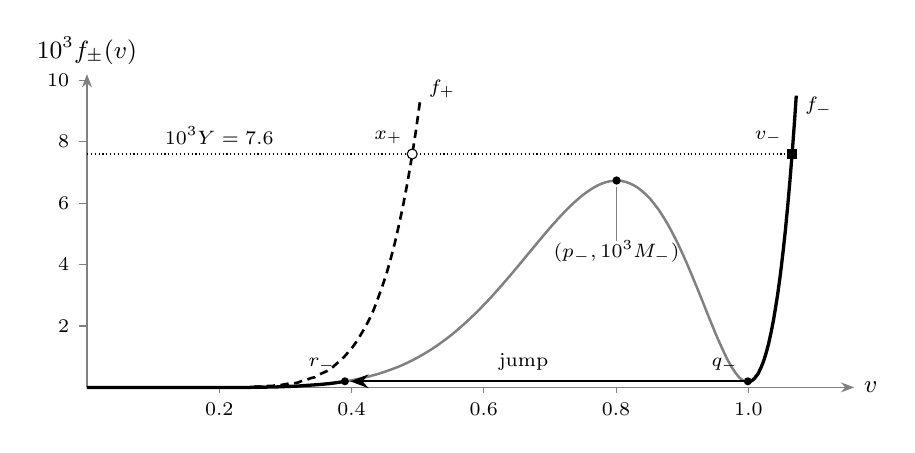
\begin{tikzpicture}[>=Stealth,font=\small,x=8.4cm,y=0.39cm]
  \draw[->,gray] (0,0) -- (1.16,0) node[right,black] {$v$};
  \draw[->,gray] (0,0) -- (0,10.2) node[above,black] {$10^3 f_\pm(v)$};
  \foreach \vx in {0.2,0.4,0.6,0.8,1.0}
    \draw[gray] (\vx,0) -- (\vx,-0.18) node[below,black,font=\scriptsize] {\vx};
  \foreach \vy in {2,4,6,8,10}
    \draw[gray] (0,\vy) -- (-0.012,\vy) node[left,black,font=\scriptsize] {\vy};
  % The form (1-v)^2+(2-a)v avoids cancellation near the minimum.
  \draw[densely dashed,line width=0.95pt] plot[domain=0:0.505,samples=80]
    (\x,{1000*(\x)^8*(1+1.9998*\x+(\x)^2)});
  \draw[line width=0.9pt,gray] plot[domain=0.390000:0.999097,samples=100]
    (\x,{1000*(\x)^8*((1-\x)^2+0.0002*\x)});
  \draw[line width=1.2pt] plot[domain=0:0.390000,samples=50]
    (\x,{1000*(\x)^8*((1-\x)^2+0.0002*\x)});
  \draw[line width=1.2pt] plot[domain=0.999097:1.073,samples=50]
    (\x,{1000*(\x)^8*((1-\x)^2+0.0002*\x)});
  \draw[densely dotted] (0,7.6) -- (1.065932,7.6);
  \node[above,font=\scriptsize] at (0.20,7.6) {$10^3Y=7.6$};
  \node[above right,font=\scriptsize] at (0.502,9.1) {$f_+$};
  \node[right,font=\scriptsize] at (1.071,9.15) {$f_-$};
  \draw[->,thick] (0.995,0.19919) -- (0.398,0.19919);
  \node[above,font=\scriptsize] at (0.66,0.23) {jump};
  \fill (0.390000,0.19919) circle (1.45pt) node[above left,font=\scriptsize] {$r_-$};
  \fill (0.999097,0.19919) circle (1.45pt) node[above left,font=\scriptsize] {$q_-$};
  \draw[thin,gray] (0.800723,4.78) -- (0.800723,6.54);
  \fill (0.800723,6.73784) circle (1.5pt);
  \node[font=\scriptsize] at (0.800723,4.42) {$(p_-,10^3 M_-)$};
  \filldraw[fill=white] (0.491683,7.6) circle (1.8pt)
    node[above left,font=\scriptsize] {$x_+$};
  \fill ([xshift=-1.7pt,yshift=-1.7pt]1.065932,7.6) rectangle ++(3.4pt,3.4pt);
  \node[above left,font=\scriptsize] at (1.065932,7.6) {$v_-$};
\end{tikzpicture}
\caption{The one-sided well at $m=8$, $a=1.9998$ and $Y=0.0076>M_-$.
The two markers on the dotted line are the roots at the comparison height.
The dashed graph contributes its full action up to $x_+$. On the solid
graph the jump from $q_-$ to $r_-$ omits the grey arc. Integrating the
squared slopes on the retained intervals gives
$-1.7\cdot10^{-5}<J_+(Y)-J_-(Y)<-1.6\cdot10^{-5}$.}
\label{fig:well}
\end{figure}

\begin{lemma}[Retained-action reversal at a one-sided well]\label{lem:well}
For every even integer $m=2d\ge 8$, there exist $a\in(0,2)$ and three regular levels $0<Y_1<Y_2<Y_3$ (outside $[\mu_-,M_-]$, with $Y_2,Y_3>M_-$) at which $J_+(Y_i)-J_-(Y_i)$ for $f_\pm$ in~\eqref{eq:well-model} has strict signs $+,-,+$, while $\int_0^\infty v\big[(w+f_+(v))^{-1}-(w+f_-(v))^{-1}\big]\,\dd v<0$ for every $w>0$.
\end{lemma}

\begin{proof}
At the limiting parameter $a=2$, $f_-(v)=v^{2d}(v-1)^2$ has its minimum $\mu_-=0$ at $q_-=1$ with inner landing $r_-=0$, and its maximum $M_-=t_*^2$ at $p_-=d/(d+1)$ where $t_*=(d/(d+1))^d/(d+1)$. Approaching $Y\downarrow M_-$ from above, the positive-side entry $x\in(0,1)$ and negative-side outer entry $v>1$ solve
\[
  x^d(1+x) = t_*,\qquad v^d(v-1) = t_*.
\]
We prove first that at $t=t_*$, the full plus action $\int_0^x f_+'(r)^2\,\dd r/r$ is strictly smaller than the retained minus outer action $\int_1^v f_-'(r)^2\,\dd r/r$.

For $d\ge 10$, vary $0<t\le t_*$ and let $x(t)\in(0,1)$, $v(t)>1$ solve $x^d(1+x)=t$ and $v^d(v-1)=t$. Since $f_+'(x)\,\dd x=2t\,\dd t$ and $f_-'(v)\,\dd v=2t\,\dd t$, differentiating the two actions with respect to $Y=t^2$ ($\dd Y=2t\,\dd t$) gives $2t\,K_+(x(t))$ and $2t\,K_-(v(t))$, where
\[
  K_+(x) = \frac{f_+'(x)}{2tx} = x^{d-2}\big(d+(d+1)x\big),\qquad
  K_-(v) = \frac{f_-'(v)}{2tv} = v^{d-2}\big((d+1)v-d\big).
\]
Since $v>1$, $K_-(v)>1^{d-2}(d+1-d)=1$ for all $0<t\le t_*$. Conversely, $K_+(x)$ increases strictly on $(0,1)$, and at $t=t_*$ we claim $x_*:=x(t_*)>2/3$: indeed for $d\ge 10$, $(2/3)^d(5/3)<1/(3(d+1))$ because $5(d+1)(2/3)^d$ decreases for $d\ge 10$ with $5\cdot 11\cdot(2/3)^{10}=56320/59049<1$, while $t_*=p_-^d/(d+1)>1/(3(d+1))$ because $(1+1/d)^d<e<3$. Using $x_*>2/3$ and $x_*^d=t_*/(1+x_*)$ gives
\[
  K_+(x_*) = \frac{t_*}{x_*^2}\!\left(d + \frac{x_*}{1+x_*}\right) < \frac{9}{4}\,\frac{p_-^d}{d+1}(d+1) = \frac{9}{4}\!\left(\frac{d}{d+1}\right)^{\!d} < 1,
\]
where the final inequality holds for all $d\ge 10$ since the first three binomial terms of $(1+1/d)^d$ equal $1+1+\frac{d-1}{2d}\ge 2+\frac{9}{20}=\frac{49}{20}>\frac{9}{4}$. Integrating $2t\,K_+(x(t))<2t<2t\,K_-(v(t))$ with respect to $Y=t^2$ from $0$ (where both actions vanish) to $t_*^2$ proves the strict inequality for all $d\ge 10$.

For the remaining degrees set $P_s(r)=\int_0^r f_s'(w)^2\,\dd w/w$ at $a=2$ and
$B_d=1-(P_-(v_*)-P_-(1))/P_+(x_*)$. In the following array an integer $j$
denotes the root interval $[j/N,(j+1)/N]$, $N=10^6$.
{\scriptsize\[
\setlength{\arraycolsep}{3pt}
\begin{array}{c|rrrrrrr}
d &3&4&5&6&7&8&9\\\hline
X &420319&484663&534554&574570&607498&635144&658736\\
V &1083024&1063933&1051986&1043803&1037847&1033317&1029755\\
100B_d & (22,23)&(-9,-8)&(-36,-35)&(-61,-60)&(-82,-81)&(-102,-101)&(-119,-118)
\end{array}
\]}
Here each $X$ satisfies $X^d(N+X)<N^{d+1}t_*<(X+1)^d(N+X+1)$.
For $V$ the same inequalities hold with $V-N$ and $V+1-N$ in the
second factors. Monotonicity gives $x_*\in[X/N,(X+1)/N]$ and
$v_*\in[V/N,(V+1)/N]$. Write $c_s=(m,2s(m+1),m+2)$.
Since $P_s(r)=\sum_{i,j=0}^2 c_{s,i}c_{s,j}r^{2m-2+i+j}/(2m-2+i+j)$
is increasing, the two rational bounds for $B_d$ are
\[
1-\frac{P_-((V+1)/N)-P_-(1)}{P_+(X/N)}
\ \le B_d\le\
1-\frac{P_-(V/N)-P_-(1)}{P_+((X+1)/N)} .
\]
Substitution gives the open intervals in the last row. The retained
minus action is larger for $4\le d\le9$. This particular endpoint
comparison reverses at $d=3$.

Fix $Y_2>M_-(2)$ slightly above $t_*^2$ so that $P_+(x(Y_2))-\big(P_-(v(Y_2))-P_-(1)\big)<0$ at $a=2$. As $a\uparrow 2$, $q_-(a)\to 1$, $\mu_-(a)\to 0$, $r_-(a)\to 0$, and $M_-(a)\to t_*^2<Y_2$, so by continuity of the roots and integrals we may fix $a\in(0,2)$ near $2$ at which $Y_2>M_-(a)$ still has $J_+(Y_2)-J_-(Y_2)<0$. At small $Y_1\in(0,\mu_-(a))$ no jump is deleted. Here $E(v)=v^m(1+v^2)\sim v^m$ as $v\downarrow0$ and $C(v)=av^{m+1}$. The moving-endpoint calculation in the proof of~\eqref{eq:tail-action}, now at zero with leading even exponent $m$ and odd exponent $m+1$, gives $J_+(Y_1)-J_-(Y_1)\sim \frac{6ma}{2m-1}Y_1^{(2m-1)/m}>0$. At large $Y_3\gg M_-(a)$ the leading even and odd exponents are $m+2$ and $m+1$. Formula~\eqref{eq:tail-action} gives $J_+(Y_3)-J_-(Y_3)\sim\frac{2(m+2)a}{2m+1}Y_3^{(2m+1)/(m+2)}>0$. Finally, $f_+(v)-f_-(v)=2av^{m+1}>0$ on $v>0$ makes $(w+f_+(v))^{-1}-(w+f_-(v))^{-1}<0$ everywhere on $v>0$ for every $w>0$.
\end{proof}

\begin{proposition}[Two-degree induction step]\label{prop:well-step}
Let $G_s=E+sC$ satisfy the hypotheses of Subsection~\ref{subsec:quad-realize} with even degree $\deg E=m\ge 8$, $[z^m]E=c>0$, highest odd degree $\deg C=m-1$, and $\sgn[z^{m-1}]C=\beta\in\{\pm 1\}$. Suppose the last outward signs of $(J_+^U-J_-^U,\,J_-^I-J_+^I,\,N)$ are $(\beta,-\beta,-\beta)$. Fix $a\in(0,2)$ from Lemma~\ref{lem:well}. Then for sufficiently large $Q>0$, the extended profiles
\begin{equation}\label{eq:well-append}
  E_{\mathrm{new}}(z) = E(z) + \frac{c}{Q^2}z^{m+2},\qquad
  C_{\mathrm{new}}(z) = C(z) - \frac{\beta ac}{Q}z^{m+1}
\end{equation}
retain all hypotheses of Subsection~\ref{subsec:quad-realize} and all fixed earlier signs, have $(\deg E_{\mathrm{new}},\deg C_{\mathrm{new}})=(m+2,m+1)$ with $\sgn[z^{m+1}]C_{\mathrm{new}}=-\beta$, add $3$ upper changes, $3$ positive-incoming changes, and $1$ negative-incoming change, and end with terminal sign triple $(-\beta,\beta,\beta)$.
\end{proposition}

\begin{proof}
Since $1-av+v^2\ge(1-a/2)(1+v^2)$ on $v\ge 0$ and lower terms satisfy $O(z^{m-1})$, $G_{s,\mathrm{new}}(z)\ge c_1 z^m(1+(z/Q)^2)$ for large $z$ uniformly in large $Q$, while $G_{s,\mathrm{new}}\to G_s$ in $C^3$ on compact sets. All earlier folds, landings, and positive samples therefore persist, and dominated convergence preserves all earlier $N(w)$ signs. Beyond a fixed compact set containing all old critical points, $G_{s,\mathrm{new}}'(z)/(cz^{m-1})=m-s\beta a(m+1)(z/Q)+(m+2)(z/Q)^2+O(1/z)$, which for large $Q$ creates \emph{only} one simple maximum and one subsequent positive minimum on side $s=\beta$ near $z/Q=p_-,q_-$ at heights $\asymp cQ^m\to+\infty$ (strictly above all old windows) and no critical points on side $s=-\beta$. Rescaling $z=Qv$ and height by $cQ^m$, $G_{s,\mathrm{new}}(Qv)/(cQ^m)\to f_{-s\beta}(v)$ in~\eqref{eq:well-model}; in action units $c^2 Q^{2m-2}$, the old bounded jump deletions cost $O(Q^{-(2m-2)})=o(1)$, so at $Y=cQ^m Y_i$ ($i=1,2,3$ from Lemma~\ref{lem:well}) $(J_+^U-J_-^U)/(c^2 Q^{2m-2})$ converges to $-\beta(J_+(Y_i)-J_-(Y_i))$, appending $-\beta(+,-,+)$ to the upper list ($3$ changes after $+\beta$) and its negative $\beta(+,-,+)$ to $J_-^I-J_+^I$ ($3$ changes after $-\beta$). At $w=cQ^m$ ($z=Qv$), $N_{\mathrm{new}}(cQ^m)/(c^{-1}Q^{2-m})$ converges by the uniform tail bound $1+(z/Q)^2$ to $-\beta\int_0^\infty v[(1+f_+)^{-1}-(1+f_-)^{-1}]\,\dd v$, which has sign $+\beta$ by Lemma~\ref{lem:well} ($1$ change after $-\beta$). The new terminal triple is $(-\beta,\beta,\beta)=(\beta_{\mathrm{new}},-\beta_{\mathrm{new}},-\beta_{\mathrm{new}})$.
\end{proof}

\subsection{Assembly at exact degree}\label{subsec:prove-asymptotic}
Write $t$ for the number of well insertions. The two assemblies also
work for $t=0$, when they use only the original seed.

\begin{proof}[Proof of Theorem~\ref{thm:main-asymptotic} and Corollary~\ref{cor:octic-low}]

Fix the profile of Lemma~\ref{lem:octic-base}, including its parameter $\eta$
and the three finite lists. For each of $t$ insertions choose the model
parameter and its regular samples first. Choose the new radius only after
fixing all earlier radii and samples. Proposition~\ref{prop:well-step}
then preserves their strict inequalities. After $t$ insertions at radii
$Q_1\ll\dots\ll Q_t$ this gives normalized profiles $(E,C)$ of degrees $(8+2t,7+2t)$ with top odd sign $\beta=(-1)^t$. At this stage:
\begin{itemize}
  \item In increasing $Y$, $J_+^U-J_-^U$ starts $+$, has $8+3t$ changes, and ends $+\beta$;
  \item In increasing $Y$, $J_-^I-J_+^I$ starts $-$, has $4+3t$ changes, and ends $-\beta$;
  \item In increasing $w>0$ (i.e.\ decreasing ordinate $-Sw$), $N(w)$ starts $-$, has $t$ changes, and ends $-\beta$.
\end{itemize}

\emph{Odd output degree.}
Let $n=11+2t$ with $t\ge0$. Keep the degrees $(m',j)=(8+2t,7+2t)$,
so $g=m'-j=1$ and $p=2-g=1$. Fix $T$ above the samples and critical
values. Proposition~\ref{prop:physical-quad} realizes all lists for the
same large $L$ at a matched upper reference $ST$. Detune its zero to
sign $-\beta$ within an arbitrarily small interval about $a_L$, keeping
the incoming signs fixed. Proposition~\ref{prop:sard}(i) gives a
polynomial $P$ with $q=9+3t$ compact hyperbolic cycles.
\hypertarget{octic-core}{At $t=0$}, $P$ itself has exact degree eight:
the eight changes from Lemma~\ref{lem:octic-base} and the detuned reference
give nine hyperbolic cycles before the exterior transfer. Its top even
coefficient is positive and its top odd coefficient $b$ has sign $\beta$.

Read the entrance ordinates in decreasing order. Reversing the positive
list preserves its $4+3t$ changes and leaves its sign at the lowest
positive ordinate equal to $-1$. The negative list begins with $-1$,
has $t$ changes and ends with $-\beta$. Thus the join adds zero changes
and the whole list has $r=4+4t$. Its last sign $-\beta$ is opposite to
the direct sign $\sgn(bp)=\beta$. Proposition~\ref{prop:cap-transfer}
therefore gives exact degree $\max(m'+2,j+4)=11+2t$ and at least
\[
                 q+r+2=(9+3t)+(4+4t)+2=15+7t
\]
simultaneous hyperbolic cycles. \hypertarget{odd-closure}{Thus $t=0$ and
$t=1$ give fifteen at degree eleven and twenty-two at degree thirteen.}

\emph{Even output degree.}
Let $n=12+2t$ with $t\ge0$. Before choosing $L$, add $\mu z^{m+2}$ to
$E$, where $m=8+2t$ and $\mu>0$ is sufficiently small. Now
$(m',j)=(10+2t,7+2t)$, $g=3$ and $p=-1$. Lemma~\ref{lem:tail-action}
preserves the finite lists. At a new large regular level
$Y_{\mathrm{far}}=E_{\mathrm{new}}(R)$, formula~\eqref{eq:tail-action}
appends $-\beta$ to the upper list and $+\beta$ to the positive
entrance list. They now have $9+3t$ and $5+3t$ changes respectively.
Use Proposition~\ref{prop:physical-quad} at a common large $L$ and
detune the upper reference to sign $+\beta$. Proposition~\ref{prop:sard}(i)
gives $q=10+3t$ compact hyperbolic cycles. At $t=0$ this intermediate
polynomial has exact degree ten and gives the ten-cycle entry of
Corollary~\ref{cor:octic-low}. As above, joining the reversed
positive list to the negative list adds zero changes. The resulting list
has $5+4t$ changes and ends with $-\beta$.

Choose a nonzero shift $\Delta$ of sign $-\beta$ small enough to keep
these strict entrance signs at every fixed ordinate. Only now append
$y_{\mathrm{tail}}=-w$ for sufficiently large $w$.
Lemma~\ref{lem:incoming-rays}(iii) gives
\[
        I_{+,P}(-w)-I_{-,P}(-w-\Delta)=-\Delta+o(1).
\]
Its sign is $+\beta$, opposite to the preceding sign and to the direct
sign $\sgn(bp)=-\beta$. Thus $r=6+4t$ and
Proposition~\ref{prop:cap-transfer} gives exact degree
$\max(m'+2,j+4)=12+2t$ and at least
\[
                  q+r+2=(10+3t)+(6+4t)+2=18+7t
\]
simultaneous hyperbolic cycles. At $t=0$ this exterior closure gives
eighteen at degree twelve. The nineteen-cycle bound in Theorem~S1.1
of the supplement uses a separate joint match.

For even $n\ge14$ take $t=(n-12)/2$, and for odd $n\ge15$ take
$t=(n-11)/2$. These substitutions give~\eqref{eq:parity-bounds},
starting with $25$ and $29$ cycles respectively. Hyperbolic persistence gives the open sets in Theorem~\ref{thm:main-asymptotic}.
\end{proof}

\section{A second construction using remote odd powers}\label{sec:remote}
A second profile construction gains fourteen cycles for every four
degrees. Each stationary inflection splits on both reflected sides.
Moment conditions at separated radii prescribe two cubic fold windows
at each inflection. A gap between the highest odd power and the even
degree allows further sign changes on the last rising branch while
the earlier samples stay fixed. Propositions~\ref{prop:physical-quad},
\ref{prop:cap-transfer} and~\ref{prop:sard} realize this single profile
and close its orbits. The resulting bounds have the same asymptotic
coefficient as Theorem~\ref{thm:main-asymptotic} and smaller finite-degree
constants.

\begin{proposition}[Cycle counts from remote powers]\label{prop:remote-odd}
For integers $h\ge1$ and $e\in\{0,1,2,3\}$ one has
\begin{equation}\label{eq:remote-formula}
 \HH(10+4h+e)\ge14h+c_e,\qquad(c_0,c_1,c_2,c_3)=(9,10,13,14).
\end{equation}
The bounds hold on nonempty open sets of exact-degree coefficients.
In particular $\HH(n)\ge(7n-63)/2$ for $n\ge14$.
\end{proposition}

\subsection{Two cubic windows at separated heights}
For real $a<0,b$, let $f(v)=v^3+av+b$, $k=\sqrt{-a/3}$,
$\mu=b-2k^3$, $M=b+2k^3$, and
\[
 P_a(v)=\int_0^v(3r^2+a)^2\,\dd r=\tfrac95v^5+2av^3+a^2v.
\]
The largest increasing inverse skips $[-2k,k]$ at $\mu$.
For $T\ne\mu,M$ let $v$ be the largest root of $f(v)=T$ and set
\begin{align}
 J^I_{a,b}(T)&=P_a(v)-\ind_{T>\mu}\{P_a(k)-P_a(-2k)\},\nonumber\\
 J^U_{a,b}(T)&=
 \begin{cases} P_a(-2k),&\mu<T<M,\\ J^I_{a,b}(T),&\text{otherwise}.
 \end{cases}                                                     \label{eq:remote-cubic}
\end{align}
The half-returns follow the original flow forward on the right and
backward on the left. In this orientation the physical ordinate, hence
the cubic height, decreases. An entrance from the right follows the
largest root in $J^I_{a,b}$. For a launch with $\mu<T<M$, the singular
launch path follows the inner rising branch. The reference follows the
outer rising branch to $v=k$ and jumps to $v=-2k$ at height $\mu$.
Just below $\mu$ both singular paths follow the inner branch with $v<-2k$.
Thus $-2k$ is the upper integration endpoint for their common segment
in $J^U_{a,b}(T)$.

\begin{lemma}[Action differences at two cubic windows]\label{lem:skew-cubic}
For every sufficiently large $C>0$, there exist $\alpha<-1$ and $\Lambda$
for which the two differences
\[
 D^X(T)-\Lambda
 =J^X_{\alpha+1,-C}(T)-J^X_{\alpha-1,C}(T)-\Lambda,\qquad X=U,I,
\]
have, at finite regular samples in increasing order, respectively seven
and three strict changes. Both lists start positive and end negative.
The samples for the two lists can be chosen independently.
\end{lemma}
\begin{proof}
Write $a_\pm=\alpha\pm1$, $k_\pm=\sqrt{-a_\pm/3}$. The windows will be
disjoint. At $M_+=-C+2k_+^3$ the upper difference jumps up by
$P_{a_+}(2k_+)-P_{a_+}(k_+)>0$. At $M_-=C+2k_-^3$ it jumps down by
the corresponding positive amount for the minus profile. We equalize the
midpoints $L_C,R_C$ of the two jumps.

Take $\alpha=-t C^{2/9}$ with $1/4\le t\le3$. For large $C$ both
$a_\pm<0$, and the two window widths are $O(C^{1/3})$. At $Y\gg|a|^{3/2}$
the positive root $v^3+av=Y$ satisfies
\begin{equation}
 P_a(v)=\tfrac95Y^{5/3}-aY+O(a^2Y^{1/3}).                     \label{eq:inverse}
\end{equation}
Indeed $v/Y^{1/3}=1-a/(3Y^{2/3})+O(a^2/Y^{4/3})$ by the implicit
function theorem at 1. Oddness gives the negative-root expansion at
large negative $Y$. At the first jump the regular minus root has
$|Y|=2C-2k_+^3$. At the second the regular plus root has
$Y=2C+2k_-^3$. All the endpoint and skip terms involving only $k_\pm$
are $O(k_+^5+k_-^5)=o(C)$. Expansion of \eqref{eq:inverse} at $2C$
therefore gives, uniformly in $t$,
\[
 \frac{R_C-L_C}{C}=
 12\,2^{2/3}(t/3)^{3/2}-4+o(1).
\]
The first term comes from the sum $2(k_-^3+k_+^3)$ of the height
increments and the second from $a_+-a_-=2$. This expression has opposite
signs at $t=1/4$ and $t=3$. Continuity in $t$ gives a common midpoint
$\Lambda\sim(9/5)(2C)^{5/3}$.

At $T=0$ both differences are asymptotic to $(18/5)C^{5/3}$. Their
ratios to $\Lambda$ tend to $2^{-2/3}<1$.
At $T=C^2$ both are asymptotic to $6CT^{2/3}$, by
\eqref{eq:inverse} at $T+C,T-C$. Here the $O(T)$ linear term, the
$O(|\alpha|^2T^{1/3})$ error and the skips are all lower order.
Thus both exceed $\Lambda$ there. With $C,\alpha$ now fixed,
$D^U,D^I=-2T+O_{C,\alpha}(|T|^{2/3})$ at either infinity.
Take successive samples far to the left, immediately before and after
$M_+$, at 0, immediately before and after $M_-$, at $C^2$, and far
to the right. These give $+,-,+,-,+,-,+,-$ for the upper difference.
The two tails, 0 and $C^2$ give $+,-,+,-$ for the incoming difference.
All samples stay off both pairs of critical values.
\end{proof}

\subsection{Simultaneous preparation at separated radii}
Write $u=z^2/2$ and fix $h\ge1$. Here $B_u$ denotes the derivative of $B(\sqrt{2u})$. Choose separated $0<q_1<\cdots<q_h$
and set
\[
 B(z)=\tfrac32 z^3\prod_{i=1}^h(1-z^2/q_i^2),\qquad
 E_0(z)=\int_0^z vB(v)^2\,\dd v,\qquad J=3+2h .
\]
We call each $q_i$ a \emph{shoulder} of the unperturbed profile.
It is a stationary inflection. The polynomial $B$ has a simple zero there, so $E_0'=zB^2$
has a double zero and $E_0'''(q_i)=2q_i B'(q_i)^2>0$. The prepared
perturbation opens a maximum and a minimum near $q_i$ on each side.
The initial even degree is $m_0=2J+2=8+4h$. Write $s_i=(-1)^i$.

\begin{lemma}[Simultaneous sign lists at separated radii]\label{lem:remote-base}
There are positive profiles $G_s=E_\eta+sC$ of the above type, of even degree
$m_0$ and highest odd degree $j_0=J+2$, with germs
\[
 E_\eta(z)=\eta z^2+O_\eta(z^8),\qquad
 C(z)=\tfrac32\eta z^3+O_\eta(z^5)
\]
for a fixed $\eta>0$. At each shoulder $q_i$ of $E_0$, in increasing order of
positive regular height, the signs of $J_+^U-J_-^U$ and $J_-^I-J_+^I$ are
\[
 s_i(+,-,+,-,+,-,+,-),\qquad -s_i(+,-,+,-),
\]
respectively. At increasing negative entrance magnitudes $w$ there are
$h+1$ alternating signs of $N(w)$ beginning negative. The leading sign
of $C$ is $\beta_0=-(-1)^h$.
\end{lemma}
\begin{proof}
Choose the radii and the odd height-splitting mode $H$ together. Write $H=z^5C_0(z^2)$ with $C_0(0)=-1$ and $\deg C_0\le h$. Require
\[
 \int_0^{q_i}B^2H'\,\dd z=0,\qquad 1\le i\le h.
\]
The prefix
integral equations are square in the remaining coefficients. Subtracting
successive equations gives one zero integral on each $(q_{i-1},q_i)$,
$q_0=0$. In the homogeneous system $H_z/z^4$, a polynomial in
$z^2$ of degree at most $h$, would have a positive root in each interval
and a root at zero. Hence the system is invertible. For its solution
the same $h$ interior roots force the top degree.

The case of zero shoulders has $B=(3/2)z^3$, $H=-z^5$.
Assume the first $i$ radii and their moment solution have been chosen. Suppose the old top terms are $b z^j$, $a z^{j+2}$, with $ab<0$.
Append $q=L$ by multiplying $B$ by $1-z^2/L^2$. In the new system
write the odd shape as an old-degree trial polynomial plus
$\lambda L^{-2}z^{j+4}$. The old rows converge to the preceding
invertible system, with zero limiting coefficient in the new column.
In the new row put $z=Lv$ and divide by $b^2 L^{3j+2}$. In the limit
the old rows have fixed the trial top coefficient at $a$, and the new
row is
\[
 \int_0^1 v^{2j}(1-v^2)^2\big((j+2)a v^{j+1}
                            +(j+4)\lambda v^{j+3}\big)\,\dd v=0.
\]
The new diagonal coefficient is positive. Thus all old coefficients
converge and $\lambda\to-aD_j$, where
\[
 D_j=\frac{(j+2)(3j+8)}{(j+4)(3j+2)}>1 .
\]
The numerator exceeds the denominator by $8$.
Consequently $H(L)/L^{j+2}\to a(1-D_j)$, of the opposite sign to $a$.
The sign of $B_z(L)$ is opposite to $b$, and the new top signs are
again opposite. Strict inequalities at earlier shoulders persist. All
limits here follow coefficientwise after the indicated substitution.

For $w>0$ write
\[
 K(w)=\int_0^\infty \frac{zB(z)}{(w+E_0(z))^2}\,\dd z .
\]
Fix the old flight samples before enlarging $L$. The new primitives and
odd shapes converge on compact sets. For large $z$ the contribution of
the old top square to the new $E_0$ equals
\[
 b^2 z^{2j+2}\left(\frac1{2j+2}-\frac{2(z/L)^2}{2j+4}
                                +\frac{(z/L)^4}{2j+6}\right).
\]
The bracket is bounded below by a positive multiple of $1+(z/L)^4$,
as follows by integrating a square or by its negative discriminant.
Every lower contribution is $O(z^{2j}(1+(z/L)^4))$ for $z\ge1$,
uniformly in $L\ge1$. The new $|B|$ is bounded by
$Cz^j(1+(z/L)^2)$. These give an integrable tail bound for every old
sample. At large $w$ the new $K$ has the sign of the new top odd
coefficient. Scaling $z=w^{1/\deg E_0}v$ in the top-degree range gives
a nonzero signed limit after division by $w^{(\deg B+2)/\deg E_0-2}$.
Bounded abscissas contribute $O(w^{-2})$. Thus the new large-$w$ sign is that of $-b$, whereas the preceding
large-$w$ sign was that of $b$. At the zero-shoulder start,
$B=(3/2)z^3$ makes the integrand of $K$ positive for every $w>0$.
Keeping each old sample before taking the next large $w$ proves the induction.

At each radius put $u_i=q_i^2/2$ and set
$b_i=|B_u(u_i)|$, $l_i=\sqrt{3/b_i}$, $d_i=b_i l_i$ and $r_i=b_i^2 l_i$.
Choose $g>0$ so that $gH(q_i)/(s_i d_i)=-C_i$ is negative of sufficiently
large magnitude at every $i$. The cubic comparison in
Lemma~\ref{lem:skew-cubic} gives $\alpha_i,\Lambda_i$ for the two graphs
$v^3+(\alpha_i\pm1)v\mp C_i$ and the two lists in the statement.
To specify their offsets on the polynomial, put
$a_{s,i}=\alpha_i+s s_i$. For $a<0$ let
\[
 p_a(v)=9v^5/5+2av^3+a^2v,\quad k=\sqrt{-a/3},\quad
 d(a)=p_a(k)-p_a(-2k).
\]

For the two even controls consider the map
\[
 {\cal L}(V)=\left((V(q_i))_{i=1}^h,
          \left(\int_0^{q_i}V B'\,\dd z\right)_{i=1}^h\right),
 \qquad V\in z^6\R_{\le 2h}[z^2].
\]
If $\mathcal L(V)=0$, divisibility at the $q_i$ and evenness give $V=BW$
with $W=z^3P(z^2)$, $\deg P\le h$. Consecutive moment differences and
$B(q_i)=B(0)=0$ give $\int_{q_{i-1}}^{q_i}B^2 W'\,\dd z=0$, $q_0=0$.
If $[z^6]V=0$ then $W=z^5P_0(z^2)$, $\deg P_0\le h-1$.
Consequently $W'/z^2$ has degree at most $h$ in $z^2$ and vanishes at zero.
Unless identically zero it also has a positive root in each of the $h$
disjoint intervals, a contradiction. Thus $W$ is zero. The restriction of $\mathcal L$ to
$\mathcal V_0=z^8\R_{\le 2h-1}[z^2]$ (zero $z^6$ coefficient) is
therefore an isomorphism onto $\R^{2h}$. The full space has dimension
$2h+1$ and its one-dimensional kernel is spanned by $B^2$, since
$\int_0^{q_i}B^2B'\,\dd z=0$. Choose $D=2+V$ with $V\in\mathcal V_0$
first, and then $Z\in\mathcal V_0$, by specifying all $2h$ coordinates
of each image:
\begin{align}
 D(q_i)&=\alpha_i b_i,& \int_0^{q_i} D B'\,\dd z&=0,\nonumber\\
 Z(q_i)&=0,&4\int_0^{q_i}(Z B'+g D H')\,\dd z
 &=\sum_{l<i}r_l\{d(a_{+,l})-d(a_{-,l})\}-s_i r_i\Lambda_i .
                                                              \label{eq:offset}
\end{align}
The constant two in $D$ supplies the quadratic germ. Its contribution
to the last row, including $2gH(q_i)$ inside the integral value, is
included when choosing $Z$.

Set $(E_\eta)_u=B^2+\eta D+\eta^{3/2}Z$, $E_\eta(0)=0$, and
$C=\eta B+g\eta^{3/2}H$. For small $z$ both $u$-slopes dominate a
positive multiple of $z^6+\eta$, since $B_u=O(z)$. At the other end
$B^2$ dominates the perturbations in leading coefficient. On intermediate
compact sets outside the roots it gives a positive slope as well. Near
$u_i$, in $u=u_i+l_i\sqrt\eta\,v$ and
$t=E_\eta(q_i)+d_i\eta^{3/2}T$, the two profiles in $T$ converge in $C^3$
on bounded $v$ intervals to
$v^3+a_{s,i}v-s s_i C_i$. Outside a large fixed multiple of $\sqrt\eta$
the quadratic growth of $B^2$ in $u-u_i$ dominates the perturbation of
the slope. This gives just two simple folds there on each side.
Their heights tend to distinct positive values for distinct $i$.
In particular the profiles are positive away from zero.

Before skips, the difference of actions up to $u_i$ is
$4\int_0^{u_i} (E_\eta)_u C_u\,\dd u$. Its terms of orders $\eta,\eta^{3/2},\eta^2$
vanish by $\int B^2 B'\,\dd z=B^3/3$ at the endpoints, the $H$ moments and
\eqref{eq:offset}. The remaining leading term is the left side of
\eqref{eq:offset} times $\eta^{5/2}$. The local primitive is
$r_i\eta^{5/2}p_{a_{s,i}}(v)+o(\eta^{5/2})$. Each earlier completed
jump deletes $r_l\eta^{5/2}d(a_{s,l})+o(\eta^{5/2})$. An axis launch
trapped inside a window uses the landing $v=-2k$, while an incoming
launch uses the largest entry root and the deletion at its minimum.
Thus \eqref{eq:offset} gives exactly the common offset of the cubic
comparison, with the physical side labels interchanged for $s_i=-1$.
All selected inequalities are strict for one sufficiently small $\eta$.
Finally $N(w)/(-2\eta)\to K(w)$ at all the finite negative samples by
dominated convergence with the weight $1+z^{m_0}$. This proves the lemma.
\end{proof}

\subsection{Adding the odd powers and closing the incoming list}
\begin{proof}[Proof of Proposition~\ref{prop:remote-odd}]
At the last shoulder of Lemma~\ref{lem:remote-base} the upper,
positive-incoming and negative-incoming lists end with signs
$(\beta_0,-\beta_0,\beta_0)$. Lemma~\ref{lem:tail-action} at
$j_0=5+2h$ gives the opposite signs farther out. Now introduce the
$h$ odd powers of degrees $j_0+2,\ldots,m_0-3$ in order. Choose each
coefficient with sign opposite to the preceding leading odd term and
small enough to preserve every sample already fixed. Only then choose
the new positive and negative ordinates far enough out to record the
next signs. Each list gains $h+1$ changes, and the final leading odd
coefficient has sign $(-1)^h\beta_0=-1$.

For $e\in\{0,1,2,3\}$ take the first $e$ terms of the ordered list
\[
  \bigl(-\delta_1 z^{m_0-1},\quad \delta_2 z^{m_0+2},\quad
        -\delta_3 z^{m_0+1}\bigr).
\]
At each step choose $\delta_i>0$ small enough to preserve the previous
samples, then select the new ordinates. Each addition switches
the relation between the current odd and even degrees from $j<m-2$
to $j=m-1$ or conversely. This adds a change to the upper and
positive-incoming lists and leaves the last negative-entrance sign
positive. With all ordinates fixed, choose the common reference and
apply Proposition~\ref{prop:physical-quad}.

Proposition~\ref{prop:physical-quad}(i) gives $\D(h_*)>0$ for a
sufficiently small $h_*>0$, preceding the negative sign at the
first shoulder. The shoulders contribute $7h$ internal changes,
and the last sign of each agrees with the first of the next. The far levels
contribute $h+1+e$ changes. Detuning the reference to the sign opposite
the last sample adds the final change. Proposition~\ref{prop:sard}(i)
then gives one linear coefficient with a simple zero in every selected
bracket, hence $q=1+7h+(h+1+e)+1=8h+3+e$ distinct compact hyperbolic cycles.

In decreasing ordinate the positive incoming list has $3h+(h+1)+e$
changes and ends positive. Its join to the first negative-ordinate
sign contributes one. The negative list has $h+(h+1)$ changes.
Thus the unshifted total is $6h+3+e$ and the final sign is positive.
For even $e$, take one sufficiently small positive $\Delta$ preserving
the whole list, then append a sufficiently negative ordinate. Indeed for
the fixed physical polynomial of even degree $m$, $I_s(-w)=w+O(w^{2/m-1})$
as $w\to\infty$ by the same positive integral equation. The translated
difference tends to $-\Delta$. This supplies one further change.
For odd $e$ take $\Delta=0$.

Use the matched-maximum theorem of Proposition~\ref{prop:cap-transfer}. For an
input of even degree $m$ and highest odd degree $j=m-g$, $g=1$ or $3$,
with top odd coefficient $b$, it gives
\[
 q+r+1+\mathbf1_{\{\sigma\ne\sgn((2-g)b)\}}
 \quad\text{at exact degree }\max(m+2,j+4).
\]
Here $r$ counts incoming changes at a single translation and $\sigma$
is the final sign. In this construction $b<0$. The final sign is
negative for $g=3$ and positive for $g=1$, so the
indicator is always one. The exact degrees and counts are
\[
\begin{array}{c|cc|cc|cc}
 e & m & j & q & r & \deg F_{\rm final}&\text{cycles}\\
 \hline
 0&m_0&m_0-3&8h+3&6h+4&m_0+2&14h+9\\
 1&m_0&m_0-1&8h+4&6h+4&m_0+3&14h+10\\
 2&m_0+2&m_0-1&8h+5&6h+6&m_0+4&14h+13\\
 3&m_0+2&m_0+1&8h+6&6h+6&m_0+5&14h+14 .
\end{array}
\]
Hyperbolic persistence gives the asserted open sets at each degree.
\end{proof}

\appendix
\section{A sharp bound in the weak full-return domain}\label{sec:weak}
Lins, de Melo and Pugh describe a Poincar\'e construction realizing
prescribed numbers of cycles for the classical equation in successive
degrees~\cite[p.~336, account of \S3]{LMP1977}. The local small-amplitude
problem for Li\'enard systems was studied by Zuppa, Blows and Lloyd,
and Christopher and Lloyd~\cite{Zuppa1981,BL1984,CL1996}.
For analytic damping Caubergh and Fran\c{c}oise give the triangular
focus quantities. Modulo the preceding generators, the first surviving
odd primitive coefficient determines the leading displacement.
Their Proposition~8, Corollary~9 and Theorems~11--12 identify the return
ideal and bound local cyclicity under the stated parameter hypotheses.
The polynomial family of Theorem~12 has zero constant damping~\cite{CF2004}.

There is already quantitative information on the return domain.
Fran\c{c}oise studies damping $\sum_{j=1}^{D}\lambda_jx^j$, whose
primitive has degree at most $D+1$ and whose constant damping vanishes.
The even damping coefficients generate his Bautin ideal. He obtains a
coefficient-weighted convergence radius and a bound for complex cycles
in an explicit disc~\cite[Theorems~1.1, 2.3 and 3.8, (3.18)]{Fr2002}.
For damping of exact degree $2\ell-1$, Caubergh and Dumortier bound
the number of cycles meeting the exterior of a sufficiently large disk
by $\ell$, uniformly on each compact coefficient family of that exact
degree. They also obtain a uniform finite bound on the total number
for such a family~\cite[Theorems~1--2]{CD2008}. Their cyclicity
estimate for the two-saddle cycle at infinity uses division and
differentiation~\cite[\S8, Theorem~9]{CD2008}.

Cao, Chen and Tang give criteria for at most two cycles on bounded
potential or half-width intervals with additional profile conditions
\cite[Theorems~1.8--1.9]{CCT2026}.

Here the linear coefficient of $F$ may vary. We bound real positive
return zeros with multiplicity on an explicit full interval of heights
for a single field by controlling the successive Wronskians there.

At height $h$ the change of coordinates $(x,y)=h(X,Y)$ sends the coefficients to
$(a_jh^{j-1})_{j=1}^n$. The following radius controls all heights of one polynomial
for which this scaled vector is small. Put
\begin{equation}\label{eq:weak-defs}
  \sigma_a(h)=\sum_{j=1}^n |a_j|h^{j-1},\quad
  \rho=2^{-(n+6)},\quad
  L_d=(d+1)!(d+1)2^d,\quad
  \delta_n=\frac{\rho^2}{72(n+2)d!\,L_d\,n^{d(d+1)/2}},
\end{equation}
where $d=\lfloor(n-1)/2\rfloor$, and denote by $\Pi_a(h)$ the first-return height from $(0,h)$ to the positive $y$-semiaxis whenever defined.

\begin{theorem}[Sharp ceiling in the weak full return]\label{thm:weak}
Let $n=\deg F\ge 1$ and $d=\lfloor(n-1)/2\rfloor$.
\begin{enumerate}
  \item[\textup{(i)}] At every height $h>0$ satisfying $\sigma_a(h)\le\delta_n$, the full return $\Pi_a(h)$ exists and depends real-analytically on $h$ and $a$.
  \item[\textup{(ii)}] If $F$ has a nonzero odd part, then $\Pi_a(h)-h$ has at most $d$ zeros across the entire set $\{h>0:\sigma_a(h)\le\delta_n\}$ in that single field, counted with multiplicity.
  \item[\textup{(iii)}] For every $n\ge 1$, the weak domain $\{h>0:\sigma_a(h)\le\delta_n\}$ can contain $d$ distinct hyperbolic limit cycles in a single field of exact degree $n$; for $n\ge 2$ the first odd perturbation in an analytic realization $F_\eps$ can be delayed to any prescribed order $\ell\ge 2$ while an even leading term enters at order~$\eps$.
\end{enumerate}
\end{theorem}

\begin{corollary}[Intrinsic orbit-damping threshold]\label{cor:intrinsic}
Put $C_n=(4n)^n/n!$ and $\kappa_n=\delta_n/(2^{n-1}C_n)$. In any single field~\eqref{eq:lienard} of exact degree $n\ge 1$, at most $\lfloor(n-1)/2\rfloor$ isolated periodic orbits $\Gamma$ satisfy $\sup_{x\in I_\Gamma}|F'(x)|\le\kappa_n$ on their own horizontal projection $I_\Gamma=x(\Gamma)$.
\end{corollary}

\noindent Thus if a field has $k>d$ isolated cycles, at least $k-d$ of
them have $|F'|>\kappa_n$ somewhere on their own horizontal projections.

\begin{lemma}[Variation kernel at a fixed reversible center]\label{prop:center-kernel}
Let $E\in\R[x]$ be an even polynomial with $E(0)=0$ whose field $X_E$ possesses a periodic orbit crossing the positive $y$-axis at $(0,H)$, $H>0$. On any nonempty open subinterval of $(0,H]$, the kernel of the first-variation operator $G\mapsto \partial_\lambda\big(\Pi_{E+\lambda G}(h)-h\big)\big|_{\lambda=0}$ on $\{G\in\R[x]:G(0)=0\}$ consists precisely of even polynomials $G$.
\end{lemma}
\subsection{Holomorphic factorization around the reversible subspace}\label{subsec:weak-factor}
Fix $n\ge 1$ and $F(x)=\sum_{j=1}^n a_j x^j$. Rescaling $(x,y)=(hX,hY)$ for $h>0$ replaces $a_j$ by $b_j=a_j h^{j-1}$ and sends $(0,h)$ to $(0,1)$. In clockwise polar coordinates $X=r\sin\theta$, $Y=r\cos\theta$, put $Q(r,\theta)=\sum_{j=1}^n b_j r^{j-1}\sin^j\theta$; then~\eqref{eq:lienard} becomes
\begin{equation}\label{eq:polar-ode}
  \dot\theta = 1 - \cos\theta\,Q(r,\theta),\qquad
  \frac{\dd r}{\dd\theta} = -\frac{r\sin\theta\,Q(r,\theta)}{1-\cos\theta\,Q(r,\theta)},\qquad r(0)=1.
\end{equation}
On the complex $\ell^1$ ball $\|b\|_1=\sum_{j=1}^n |b_j|<\rho=2^{-(n+6)}$ and the disk $|r|\le 2$, we have $|Q(r,\theta)|\le 2^{n-1}\|b\|_1<2^{-7}=1/128$ for all $\theta\in[0,2\pi]$, hence $|1-\cos\theta\,Q|\ge 127/128$ and $|\dd r/\dd\theta|\le 2(1/128)/(127/128)=2/127$. Continuation over $\theta\in[0,2\pi]$ keeps $|r(\theta)-1|\le 4\pi/127<1/4$, well inside $|r|\le 2$. Write $D(b)=r(2\pi;b)-1$ for the scaled displacement over a full turn.
The earlier $\D(h)$ compares the two half-return magnitudes.
By holomorphic parameter dependence for regular ODEs, $D$ is holomorphic on $\{\|b\|_1<\rho\}$ with $|D(b)|<1/4$. For real $b$ in this ball, $\dot\theta\ge 127/128>0$, so the scaled orbit completes one clockwise turn to $\theta=2\pi$ and
\begin{equation}\label{eq:disp-scale}
  \Pi_a(h) - h = h\,D\!\left((a_j h^{j-1})_{j=1}^n\right).
\end{equation}

\paragraph{Reversible periodic orbits.} Suppose $F$ is an even polynomial (at \emph{any} amplitude, not necessarily inside $\|b\|_1<\rho$). The reflection $S(x,y)=(-x,y)$ satisfies $X_F(S(x,y))=-DS\,X_F(x,y)$ because $F(-x)=F(x)$. Every forward right-half-plane arc from $(0,h)$ that reaches $(0,-w)$ ($w>0$) therefore closes into a periodic orbit when followed by its time-reversed reflection in $x<0$; since both axis hits $(0,h)$ and $(0,-w)$ are transverse, every nearby height $h'$ also reaches $\Sigma_-$ and closes by reflection. Taking a periodic orbit $\Gamma$ of $X_F$, Lemma~\ref{lem:half-returns}(i) gives its unique positive-$y$ crossing $(0,h)$, and its forward arc hits $\Sigma_-$ before returning (its $y$-minimum is negative on $x=0$ and $\Gamma$ meets $\Sigma_+$ only once), so $\Gamma$ lies in an open period annulus. 

In particular, for every real even vector $b_{\mathrm{ev}}$ in $\{\|b\|_1<\rho\}$ (meaning $b_{2k+1}=0$ for all $k$), $D(b_{\mathrm{ev}})=0$, which extends to all complex even vectors in $\{\|b\|_1<\rho\}$ by the identity theorem. Write $b=b_{\mathrm{ev}}+b_{\mathrm{od}}$ where $b_{\mathrm{od}}$ retains the odd indices $2k+1$ ($0\le k\le d=\lfloor(n-1)/2\rfloor$). Differentiating~\eqref{eq:polar-ode} with respect to $b_j$ at $b=0$ (where $r\equiv 1$) gives $\partial_{b_j}r(2\pi;0)=-\int_0^{2\pi}\sin^{j+1}\theta\,\dd\theta$, which vanishes for even $j$ and equals $-2\pi c_k$ for $j=2k+1$, where
\begin{equation}\label{eq:sine-moments}
  c_k = \frac{1}{2\pi}\int_0^{2\pi}\sin^{2k+2}\theta\,\dd\theta = 4^{-(k+1)}\binom{2k+2}{k+1} > 0.
\end{equation}
Integrating along the segment $s\mapsto b_{\mathrm{ev}}+s b_{\mathrm{od}}$ ($s\in[0,1]$) from $D(b_{\mathrm{ev}})=0$ yields the exact holomorphic factorization
\begin{equation}\label{eq:D-factor}
  D(b) = \sum_{k=0}^d b_{2k+1} G_{2k+1}(b),\qquad
  G_{2k+1}(b) = \int_0^1 (\partial_{b_{2k+1}}D)(b_{\mathrm{ev}}+s b_{\mathrm{od}})\,\dd s,
\end{equation}
with $G_{2k+1}(0)=-2\pi c_k$. For $\|b\|_1\le\rho/2$, varying one coordinate $b_i$ on a complex disk of radius $\rho/4$ stays inside $\{\|\tilde b\|_1<3\rho/4<\rho\}$ where $|D|<1/4$; Cauchy's integral estimate gives $|\partial_{b_i}D|\le (1/4)/(\rho/4)=1/\rho$ on $\{\|b\|_1\le\rho/2\}$, hence $|G_{2k+1}(b)|\le 1/\rho$ there. Applying Cauchy's estimate a second time on coordinate disks of radius $\rho/4$ around points of $\{\|b\|_1\le\rho/4\}$ gives $|\partial_{b_i}G_{2k+1}|\le 4/\rho^2$ on $\{\|b\|_1\le\rho/4\}$. Integrating along the ray from $0$ to $b$ in the $\ell^1$ norm yields
\begin{equation}\label{eq:G-lip}
  |G_{2k+1}(b) - G_{2k+1}(0)| \le \frac{4\|b\|_1}{\rho^2}\qquad (\|b\|_1\le\rho/4).
\end{equation}

\begin{remark}[First nonzero odd jet]\label{rem:odd-jet}
If $a(\eps)$ depends analytically on $\eps$ near $0$ with $F_0=0$ and its first nonzero odd coefficient polynomial $O(x)=\sum_{k=0}^d o_{2k+1}x^{2k+1}$ enters at order $\eps^\ell$ ($\ell\ge 1$), then~\eqref{eq:disp-scale}--\eqref{eq:G-lip} give $(\Pi_{a(\eps)}(h)-h)/h=-2\pi\eps^\ell\sum_{k=0}^d c_k o_{2k+1}h^{2k}+O_R(\eps^{\ell+1})$ uniformly on $0<h\le R$: all earlier even jets contribute identically zero to the displacement. In particular, for $F_\eps=\eps f$, cancellation of the first-order displacement on an open height interval forces every odd coefficient of $f$ to vanish.
\end{remark}

\subsection{Counting zeros on the whole height interval}\label{subsec:weak-wronskian}

\begin{proof}[Proof of Theorem~\ref{thm:weak}\textup{(i),(ii)}]
Since $\delta_n<\rho/12<\rho$ in~\eqref{eq:weak-defs}, part~(i) already holds on $\{h>0:\sigma_a(h)\le\delta_n\}$, which, when nonempty, is an interval $(0,h_{\max}]$ or $(0,\infty)$ because $\sigma_a(h)$ is nondecreasing in $h>0$. Assume $F$ has a nonzero odd part. Setting $h=e^t$ ($t\in\R$ with $\sigma_a(e^t)\le\delta_n$), formulas~\eqref{eq:disp-scale} and~\eqref{eq:D-factor} write $(\Pi_a(e^t)-e^t)/e^t=\sum_{k=0}^d a_{2k+1} f_k(t)$, where
\[
  f_k(t) = e^{2kt} G_{2k+1}\!\left((a_j e^{(j-1)t})_{j=1}^n\right),\qquad 0\le k\le d.
\]
We prove that for every $1\le q\le d+1$, the Wronskian $W(f_0,\dots,f_{q-1})(t)=\det\big(f_k^{(r)}(t)\big)_{0\le r,k<q}$ is nonzero at every real $t$ with $\sigma:=\sigma_a(e^t)\le\delta_n$.

Fix such a real $t$. On the complex disk $|\zeta|\le 1/n$, since $j-1\le n-1$ and $2k\le n-1$, we have $|e^{(j-1)\zeta}|\le e^{(n-1)/n}<3$ and $|e^{2k\zeta}|\le e^{(n-1)/n}<3$. Hence $\|b(e^{t+\zeta})\|_1\le 3\sigma\le 3\delta_n<\rho/4$. Writing $f_k(t+\zeta)=e^{2kt}\big[G_{2k+1}(0)e^{2k\zeta}+e^{2k\zeta}\big(G_{2k+1}(b(e^{t+\zeta}))-G_{2k+1}(0)\big)\big]$, estimate~\eqref{eq:G-lip} bounds the holomorphic remainder inside the bracket on $|\zeta|\le 1/n$ by $3\cdot 4(3\sigma)/\rho^2=36\sigma/\rho^2$. Applying Cauchy's derivative bound of order $r\le d$ at $\zeta=0$ on the disk of radius $1/n$ shows that after dividing column $k$ of $W(f_0,\dots,f_{q-1})(t)$ by $e^{2kt}G_{2k+1}(0)$ and row $r$ by $n^r$, the $(r,k)$ entry $M_{r,k}$ differs from $(2k/n)^r$ by at most
\[
  \eta := \frac{36\,r!\,\sigma}{|G_{2k+1}(0)|\,\rho^2} \le \frac{36(n+2)d!\,\sigma}{\rho^2},
\]
where we used $2\pi c_k>4^{-(k+1)}\binom{2k+2}{k+1}\ge 1/(2k+3)\ge 1/(n+2)$ because the central binomial coefficient is at least the average of the $2k+3$ binomial coefficients in row $2k+2$, whose sum is $4^{k+1}$. By~\eqref{eq:weak-defs}, $\eta\le 1/\big(2L_d n^{d(d+1)/2}\big)<1$. The limiting $q\times q$ Vandermonde determinant is
\[
  \det\!\left(\Big(\frac{2k}{n}\Big)^r\right)_{0\le r,k<q} = \prod_{0\le i<k<q}\frac{2(k-i)}{n} \ge n^{-q(q-1)/2} \ge n^{-d(d+1)/2},
\]
and every limiting entry satisfies $|(2k/n)^r|\le 1$. In each of the $q!$ permutation products of $\det M$, telescoping $\prod_{r=0}^{q-1} M_{r,\pi(r)} - \prod_{r=0}^{q-1}(2\pi(r)/n)^r$ bounds the total determinant perturbation by $q!\,q(1+\eta)^{q-1}\eta \le (d+1)!(d+1)2^d\eta = L_d\eta \le \tfrac12 n^{-d(d+1)/2}$, at most half the Vandermonde lower bound. Thus $\det M\neq 0$, and since $e^{2kt}G_{2k+1}(0)\neq 0$, $W(f_0,\dots,f_{q-1})(t)\neq 0$ for all $1\le q\le d+1$ (extending slightly past $h_{\max}$ by continuity so any zero at $h_{\max}$ lies inside an open nonvanishing Wronskian interval).

Now factor $f_0\neq 0$ out of $W(f_0,\dots,f_s)$: multilinearity and column expansion along the first column $(1,0,\dots,0)^\top$ give $W\big((f_1/f_0)',\dots,(f_s/f_0)'\big)=W(f_0,\dots,f_s)/f_0^{s+1}\neq 0$. By induction on $d$ using Rolle's theorem with multiplicities after dividing by $f_0$, any nontrivial linear combination $\sum_{k=0}^d a_{2k+1} f_k(t)$ has at most $d$ real zeros counted with multiplicity on the admissible $t$-interval. Since $h\mapsto\log h$ is a real-analytic diffeomorphism and the prefactor $h=e^t$ is positive, $\Pi_a(h)-h$ has at most $d$ zeros counted with multiplicity on $\{h>0:\sigma_a(h)\le\delta_n\}$.
\end{proof}

\begin{proof}[Proof of Corollary~\ref{cor:intrinsic}]
Let $\Gamma$ be an isolated periodic orbit of~\eqref{eq:lienard} satisfying $\sup_{x\in I_\Gamma}|F'(x)|\le\kappa_n$. Set $A=\max_{(x,y)\in\Gamma}|x|>0$ and pick $s\in\{\pm 1\}$ with $sA\in I_\Gamma$. Since $(0,0)$ lies inside $\Gamma$, $[0,sA]\subset I_\Gamma$, so for every $t\in[0,1]$ the mean value theorem gives $|F(sAt)/A|\le t\sup_{I_\Gamma}|F'|\le\kappa_n$. Interpolating the polynomial $p(t)=F(sAt)/A=\sum_{j=1}^n (a_j s^j A^{j-1})t^j$ of degree at most $n$ at the $n+1$ nodes $t_i=i/n$ ($0\le i\le n$), each linear factor $nt-m$ ($m\neq i$) in the numerator of the $i$-th Lagrange basis polynomial $\ell_i(t)=\prod_{m\neq i}\frac{nt-m}{i-m}$ has coefficient $\ell^1$ sum $n+m\le 2n$, so $\|\ell_i\|_1\le\frac{(2n)^n}{i!(n-i)!}$; summing over $0\le i\le n$ gives $\sum_{i=0}^n\|\ell_i\|_1\le \frac{(2n)^n}{n!}\sum_{i=0}^n\binom{n}{i}=\frac{(4n)^n}{n!}=C_n$. Hence $\sigma_a(A)=\|p\|_1\le C_n\sup_{[0,1]}|p|\le C_n\kappa_n$. At the horizontal extremum $(sA,y_*)\in\Gamma$, $\dot x=0$ forces $y_*=F(sA)$, so $|y_*|/A\le\kappa_n<1/2$; rescaling~\eqref{eq:polar-ode} by $A$ instead of $h$ starts at radius $r_*\le\sqrt{1+\kappa_n^2}<3/2$ with $\|b(A)\|_1=\sigma_a(A)<\rho$, so $|\dd r/\dd\theta|\le 2/127$ up to the positive-$y$ crossing $(0,h_\Gamma)$ keeps $h_\Gamma/A<3/2+2\pi(2/127)<2$, i.e., $h_\Gamma<2A$. Therefore $\sigma_a(h_\Gamma)\le 2^{n-1}\sigma_a(A)\le 2^{n-1}C_n\kappa_n=\delta_n$. Every such orbit $\Gamma$ thus crosses $\Sigma_+$ inside $\{h>0:\sigma_a(h)\le\delta_n\}$, where Theorem~\ref{thm:weak}(ii) bounds the total count by $d$.
\end{proof}

\begin{proof}[Proof of Lemma~\ref{prop:center-kernel}]
By Lemma~\ref{lem:half-returns}(i) and reflection across the vertical axis, every $h\in(0,H]$ closes into an even-symmetric periodic orbit of $X_E$ whose right half-arc reaches $\Sigma_-$ transversely (any right arc failing to hit $\Sigma_-$ stays bounded inside the outer orbit $\Gamma_H$ and cannot approach $(0,0)$ since $E(x)=O(x^2)$ gives $E'(0)=0$, hence polar speed $\dot\varphi\to -1$). Thus $\Pi_{E+\lambda G}(h)$ is real-analytic in $(h,\lambda)$ on $(0,H]\times(-\lambda_0,\lambda_0)$ for small $\lambda_0$ on each compact subinterval of $(0,H]$, with $\Pi_{E+\lambda G}(h)\equiv h$ whenever $G$ is even. Conversely, if $G(0)=0$ has a nonzero odd part with lowest odd term $g_{2k+1}x^{2k+1}$ ($g_{2k+1}\neq 0$), choose $N\ge\max(\deg E,\deg G)$ and apply~\eqref{eq:disp-scale}--\eqref{eq:G-lip} at degree cutoff $N$ for sufficiently small $h>0$, where $\sigma_E(h)=O(h)\to 0$ because $E(x)=O(x^2)$ has zero linear term. Differentiating $\lambda\mapsto h D\big(((e_j+\lambda g_j)h^{j-1})_{j=1}^N\big)$ at $\lambda=0$ using $D(b_{\mathrm{ev}})\equiv 0$ and $G_{2m+1}(b_E(h))=-2\pi c_m+O(h)$ gives
\[
  \left.\partial_\lambda\big(\Pi_{E+\lambda G}(h)-h\big)\right|_{\lambda=0} = \sum_{m\ge k} g_{2m+1} h^{2m+1} G_{2m+1}(b_E(h)) = -2\pi c_k g_{2k+1} h^{2k+1} + o\!\left(h^{2k+1}\right) \neq 0
\]
as $h\downarrow 0$. Since $h\mapsto\partial_\lambda(\Pi_{E+\lambda G}(h)-h)|_{\lambda=0}$ is real-analytic on $(0,H]$, it cannot vanish on any nonempty open subinterval of $(0,H]$.
\end{proof}

\subsection{Attainment with a delayed odd perturbation}\label{subsec:weak-sharp}

\begin{proof}[Proof of Theorem~\ref{thm:weak}\textup{(iii)}]
For $n=1$ ($d=0$), $F(x)=\eps x$ with $0<\eps<\delta_1$ has $\sigma_a(1)=\eps<\delta_1$ and zero closed orbits. For $n\ge 2$ and any integer $\ell\ge 2$, choose $0<h_1<\dots<h_d<R=1$ (empty if $n=2$, $d=0$) and put $q(u)=\prod_{i=1}^d(u-h_i^2)=\sum_{k=0}^d q_k u^k$. Define
\begin{equation}\label{eq:weak-realize}
  F_\eps(x) = \eps x^{2\lfloor n/2\rfloor} + \eps^\ell\sum_{k=0}^d \frac{q_k}{c_k}\,x^{2k+1}\qquad (\eps>0).
\end{equation}
Since $q_d=1\neq 0$, the highest even and odd powers of $F_\eps$ are $2\lfloor n/2\rfloor$ and $2d+1=2\lfloor(n-1)/2\rfloor+1$, whose maximum is identically $n$ for every $\eps>0$. By~\eqref{eq:disp-scale}--\eqref{eq:G-lip}, for $\eps>0$ small enough that $\sigma_{F_\eps}(1)\le\delta_n$, we have
\begin{equation}\label{eq:weak-cauchy-err}
  \left|\frac{\Pi_{F_\eps}(h)-h}{h\eps^\ell} + 2\pi q(h^2)\right| \le \frac{4\,\sigma_{F_\eps}(h)}{\rho^2}\sum_{k=0}^d\left|\frac{q_k}{c_k}\right|h^{2k} = O(\eps)\qquad (0<h\le 1).
\end{equation}
On $d$ disjoint brackets $[h_i-\nu,h_i+\nu]\subset(0,1)$ around the simple roots $h_i$ of $q(h^2)$, $\Pi_{F_\eps}(h)-h$ therefore has opposite strict endpoint signs simultaneously for one small $\eps>0$. Since the total zero multiplicity on $(0,1]$ is at most $d$ by Theorem~\ref{thm:weak}(ii), each bracket contains \emph{exactly one} zero, which must be simple. By~\eqref{eq:polar-ode}, the scalar angular variational equation gives $\Pi_{F_\eps}'(h)>0$, so simplicity $(\Pi_{F_\eps}-I)'(r_i)\neq 0$ implies $\Pi_{F_\eps}'(r_i)\neq 1$, giving $d$ simultaneous hyperbolic limit cycles inside $\{h>0:\sigma_{F_\eps}(h)\le\delta_n\}$ (and satisfying Corollary~\ref{cor:intrinsic} for small $\eps$).
\end{proof}

\begin{remark}[Dilation]
For $B(0)=B'(0)=0$ set $F_\eps(x)=B(\eps x)/\eps$.
Its coefficients tend to zero. The map $(x,y)\mapsto(\eps x,\eps y)$
takes its field to that of $B$, preserving multipliers. An orbit at height
$H$ for $B$ has height $H/\eps$ for $F_\eps$ and
$\sigma_{F_\eps}(H/\eps)=\sigma_B(H)$. Thus a cycle outside the weak
domain stays outside under dilation.
\end{remark}

\section{The split-cubic comparisons for the octic seed}\label{app:cubic}
\subsection{Retained actions of a split stationary inflection}\label{subsec:cubic}
The same pair of cubic graphs describes the splitting inflection in the octic and sextic-based constructions. The truncation at an inner landing affects only launches inside an open fold window.

For $a=-3k^2<0$ ($k=\sqrt{-a/3}>0$) and $b\in\R$, the cubic $f(v)=v^3+av+b$ has a local maximum $M=b+2k^3$ at $v=-k$, a local minimum $\mu=b-2k^3$ at $v=k$, and rising-branch landing $v=-2k$ solving $f(-2k)=\mu$. Let $P_a(v)=\int_0^v (3r^2+a)^2\,\dd r=\tfrac95 v^5+2av^3+a^2v$, which is strictly increasing on $\R$ since $P_a'(v)=(f'(v))^2\ge 0$. For $\xi\notin\{\mu,M\}$, let $v(\xi)$ be the largest real root of $f(v)=\xi$, and define the incoming and upper cubic actions
\begin{equation}\label{eq:cubic-actions}
  J_{a,b}^I(\xi) = P_a(v(\xi)) - \ind_{\{\xi>\mu\}}\big(P_a(k)-P_a(-2k)\big),\qquad
  J_{a,b}^U(\xi) = \begin{cases}
    P_a(-2k), & \mu<\xi<M,\\
    J_{a,b}^I(\xi), & \xi\notin[\mu,M].
  \end{cases}
\end{equation}
Put $\Lambda=493/2$ and define the equal-weight cubic differences
\begin{equation}\label{eq:D-cub}
  D_{\mathrm{cub}}^X(\xi) = J_{-1,-8}^X(\xi) - J_{-3,8}^X(\xi) - \frac{493}{2},\qquad X\in\{U,I\}.
\end{equation}

\begin{lemma}[Certified signs of the split-cubic comparison]\label{lem:cubic-table}
At the eight rational levels $\xi_0<\dots<\xi_7$ in Table~\ref{tab:cubic}, every $\xi_m$ lies outside both critical sets $\{\mu_\pm,M_\pm\}$ of $f_+(v)=v^3-v-8$ ($[\mu_+,M_+]=[-8-\tfrac{2}{3\sqrt3},-8+\tfrac{2}{3\sqrt3}]\approx[-8.3849,-7.6151]$) and $f_-(v)=v^3-3v+8$ ($[\mu_-,M_-]=[6,10]$), and $D_{\mathrm{cub}}^U(\xi_m)$ belongs to the listed open rational intervals, alternating $+,-,+,-,+,-,+,-$ ($7$ changes). Moreover, at the four indices $m\in\{0,3,6,7\}$ ($\xi\in\{-12,0,100,10^5\}$), $\xi_m\notin[\mu_+,M_+]\cup[\mu_-,M_-]$, so $D_{\mathrm{cub}}^I(\xi_m)=D_{\mathrm{cub}}^U(\xi_m)$ alternates $+,-,+,-$ ($3$ changes).
\end{lemma}

\begin{table}[ht]
\centering\scriptsize\setlength{\tabcolsep}{3.5pt}
\caption{Certified open rational enclosures for $D_{\mathrm{cub}}^U(\xi)$ in~\eqref{eq:D-cub}. At $\xi\in\{-12,0,100,10^5\}$, $D_{\mathrm{cub}}^I(\xi)=D_{\mathrm{cub}}^U(\xi)$ satisfies the identical enclosure. The integers specify the root brackets in the proof; L denotes the inner landing.}\label{tab:cubic}
\smallskip
\begin{tabular}{@{}lrrrrrrrr@{}}
\toprule
$\xi$ & $-12$ & $-7.62$ & $-7.61$ & $0$ & $9.99$ & $10.01$ & $100$ & $10^5$ \\
\midrule
$j_+$ & $-179633$ & L & $115639$ & $216631$ & $274737$ & $274829$ & $483219$ & $4642430$ \\
$j_-$ & $-308086$ & $-289690$ & $-289645$ & $-249204$ & L & $200111$ & $473570$ & $4643619$ \\
Lower bound & $81$ & $-0.85$ & $0.40$ & $-79$ & $21$ & $-0.43$ & $610$ & $-98000$ \\
Upper bound & $82$ & $-0.82$ & $0.44$ & $-77$ & $23$ & $-0.40$ & $615$ & $-96000$ \\
Sign of $D_{\mathrm{cub}}^U(\xi)$ & $+$ & $-$ & $+$ & $-$ & $+$ & $-$ & $+$ & $-$ \\
Sign of $D_{\mathrm{cub}}^I(\xi)$ & $+$ &  &  & $-$ &  &  & $+$ & $-$ \\
\bottomrule
\end{tabular}
\end{table}


\begin{proof}
Take $N=10^5$. Squaring gives $57735/N<k_+=1/\sqrt3<57736/N$,
and $k_-=1$. From $M=b+2k^3$, $\mu=b-2k^3$ we obtain
$\mu_+\in(-8.385,-8.384)$, $M_+\in(-7.616,-7.615)$, and
$[\mu_-,M_-]=[6,10]$. For each integer $j_s$ in the table,
\[
 f_s(j_s/N)<\xi<f_s((j_s+1)/N).
\]
Both ends lie on the increasing outer branch above the window, or on
the increasing inner branch below it. These rational comparisons
enclose the required root. To read off the action, use $P_a$ at the two
endpoints. Above the window subtract
$P_a(k)-P_a(-2k)=162k^5/5$ from both bounds, using the indicated
enclosure of $k$ outwards. Below it use $P_a$ directly. At L an upper
launch reaches the inner landing and contributes $P_a(-2k)=-138k^5/5$.
Subtract the minus interval from the plus interval and then subtract
$493/2$ as in~\eqref{eq:D-cub}. For example at $-7.62$ the plus
contribution is the landing value and the minus root lies between
$-289690/N$ and $-289689/N$. The resulting interval lies inside
$(-0.838,-0.832)$. The same endpoint substitutions give the two bound
rows. At the four indicated levels both launches retain identical
pieces on each side.
\end{proof}

\section*{Declaration of generative AI and AI-assisted technologies in manuscript preparation}
The author used OpenAI 6.2 Astra (via Codex) to explore candidate constructions, develop and check parts of the proofs, write reproducibility code, and revise the manuscript. Google Gemini 4 Carbon was used to critique draft manuscripts and identify issues in the arguments, presentation, and references. The author reviewed and revised the resulting material and takes full responsibility for the final manuscript.

\providecommand{\doilink}[1]{\href{https://doi.org/#1}{\nolinkurl{#1}}}
\begingroup
\small\raggedright
\bibliographystyle{abbrv}
\bibliography{references}
\endgroup

\end{document}
